\documentclass{article}
\usepackage{lmodern} % Latin Modern (a cleaner, scalable version of Computer Modern)
\usepackage{array}
\usepackage{amsmath}   % For all your fixed-point math formulas
\usepackage{xcolor}    % Great for adding subtle colors to your code
\usepackage{booktabs}
\usepackage{microtype}
\usepackage{enumitem}
\usepackage{tabularx}
\usepackage{booktabs} % Highly recommended for professional manual tables
\usepackage{longtable}
\usepackage[hypertexnames=false]{hyperref}
\usepackage{xurl}
\usepackage{tikz}
\usepackage{epigraph}

% Customize the epigraph layout parameters
\setlength{\epigraphwidth}{0.65\textwidth}
%\setlength{\epigraphrule}{0pt} % Removes the divider line for a cleaner look

% Define a custom command to draw the crossed/X'ed box with a subtle nudge
\newcommand{\xbox}{%
  \raisebox{-1pt}{%
    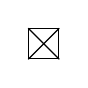
\begin{tikzpicture}
      \node[inner sep=0pt, minimum size=3.8mm, draw] (char) {};
      \draw (char.south west) -- (char.north east);
      \draw (char.south east) -- (char.north west);
    \end{tikzpicture}%
  }%
}

% Define an empty box of the exact same size, lifted by the same amount
\newcommand{\emptybox}{%
  \raisebox{-1pt}{%
    \begin{tikzpicture}
      \node[inner sep=0pt, minimum size=3.8mm, draw] (char) {};
    \end{tikzpicture}%
  }%
}

\title{$\sqrt{Eurocomp}$ LGP-21 Subroutine Handbook}
\author{Equinox Deschanel}
\date{June 2026}

\begin{document}

\maketitle

\begin{titlepage}
\clearpage\thispagestyle{empty}
\vspace*{\fill}

\epigraph{``Our need will be the real creator.''}{--- Plato, \textit{The Republic}}

\vspace{1.5em}

\epigraph{``The enemy of art is the absence of limitations.''}{--- Orson Welles}

\vspace*{\fill}
\clearpage
\end{titlepage}

\tableofcontents
\newpage
\section{Notes on the Translation}
\subsection{Number representation}
\subsubsection*{Introduction to fractional fixed-point architecture}
The LGP-21's number representation is very different from 21st century computing platforms. It is not at all unique; many early computers used it, including the IBM 701\cite{ibm701manual}, the ILLAC I\cite{illiac1954}, the Elliot 405\cite{elliott405}, the RPC-4000\cite{rpc4000manual}, and the LGP-21's predecessor, the LGP-30\cite{lgp30programmingmanual}. This architecture is known as the IAC architecture, and was first proposed by John von Neumann for EDSAC\cite{vonneumann1945first}.

A fixed-point fractional representation treats all numbers as fractions lying between $-1$ and $+1$. As von Neumann pointed out\cite{burks1946preliminary}, the multiplication of 2 $n$-bit integers results in a value that may require $2n$ bits to represent it, which could easily overflow a register, but the multiplication of \emph{fractions} always results in a number no larger, and usually smaller, than both multiplicands (e.g., $0.5 \times 0.5 = 0.25$). The answer still requires $2n$ bits to represent, but the extra bits end up in the \emph{least} significant digits, preventing overflow from occurring.

The design uses a combined register pair to contain the $2n$ bits; on the LGP-21, the accumulator receives the most significant half, and a hidden register not available to the programmer gets the least significant half. To reduce complexity, the LGP-21 simply throws this second half away. Since these are the least significant digits, the (unscaled) error introduced is $2^{-31}$ or less.

This advantage in multiplication is offset by a problem this creates with division: fractional multiplication \emph{shrinks} numbers, but fractional division (potentially) \emph{expands} them.

In a fractional fixed-point architecture, dividing two numbers requires that the absolute magnitude of the divisor has to be \emph{strictly greater than} the absolute magnitude of the dividend.$$\left| \text{Divisor} \right| > \left| \text{Dividend} \right|$$Getting this wrong means that the theoretical quotient is $\ge 1.0$, and such a value cannot physically fit in the accumulator. The architecture maintains the \emph{hardware} binary point just after the sign bit, so a value $\ge 1.0$ results in an overflow.

Von Neumann wrote that ``\emph{[t]he programmer must see to it} [emphasis mine - ED] that the left-shift [scale factor] is sufficiently large to ensure this inequality.''burks1946preliminary\cite{burks1946preliminary} The cognitive load of remembering where the \emph{implied} binary point is (via the scaling factor) vs. the \emph{physical} binary point (implemented by the hardware) is placed solely on the programmer.

Modern embedded systems use similar notation (referred to as \emph{Q-notation} or \emph{fixed-point scaling}) to define this manual placement of the implicit binary point within a computer word, and in fact, the original version of this document specifically refers to the scaling factor as $q$.

\subsubsection*{LGP-21 Fractional Fixed-point Implementation}
\label{sec:fractional-fixed-point}
The LGP-21 treats all 31-bit words strictly as fractions ranging from $-1$ to $+1$, with the physical binary point fixed immediately to the right of the (leftmost) sign bit. To work with integers or mixed numbers, the programmer must mentally shift this binary point to the right by $n$ bits (as indicated by the $@n$ notation). 

For example, a value at texttt{@3} allocates 3 bits for the integer portion of a number (allowing values up to $7.999999$) and the remaining 27 bits for the fraction. As noted above, the programmer is \emph{entirely responsible} for tracking this scale factor across operations, and must manually shift, multiply, or divide intermediate values as needed to maintain the desired scale factor.

\subsubsection*{Addition/Subtraction Pitfalls}
Addition and subtraction require that the scale factors (\texttt{@n}) of both operands be identical before the operation is executed. The LGP-21 treats every 31-bit word as a raw fixed-point fraction. If you add two numbers with different $q$ factors without shifting them appropriately, the machine will blindly align their bits and perform the operation, smashing incommensurate units of completely different mathematical weights into the same columns. 

    For example, if you attempt to add $1.0$ scaled at $\texttt{@1}$ to $1.0$ scaled at $\texttt{@4}$ without normalizing them first:
    \begin{center}
    \begin{tabular}{rrc}
        $1.0 \text{ at } \texttt{@1} \rightarrow$ & \texttt{0 100000...} & (Hardware sees $2^{29}$) \\
        $+ \quad 1.0 \text{ at } \texttt{@4} \rightarrow$ & \texttt{0 000100...} & (Hardware sees $2^{26}$) \\ \hline
        \text{Raw Sum} $\rightarrow$ & \texttt{0 100100...} & (Hardware sees $2^{29} + 2^{26}$)
    \end{tabular}
    \end{center}
Depending on which scale factor you \emph{think} the result is in, your answer is now either $1.125$ (if you assume the result is $\texttt{@1}$) or $9.0$ (if you assume $\texttt{@4}$). The machine will not throw an error, trigger an overflow, or warn you; it will simply calculate perfectly represented garbage because the binary point in the two numbers is in \emph{two different places}.
 
It is vital to understand that the LGP-21 hardware itself does not know about scale factors and has no way to check them or track them.  Scale factor changes occur during multiplication and division: multiplication \emph{adds} the scale factors, and division \emph{subtracts} them. After a multiplication or division, the result must be shifted left or right to ensure that the result conforms to the scale factor desired.

As an example, if an \texttt{@1} value were to be divided by an \texttt{@9} one, the resulting scale factor would be $-8$, meaning that to return it to an \texttt{@1} value, the result would need to be shifted right \emph{8} bits, and for an \texttt{@9} result, it would need to be shifted right \emph{17}(!) bits.

In the subroutines documented below, I've carried over the original \texttt{@n} notation where it was used, most often for referring to values in storage (e.g., $\theta@9$) or the accumulator (accumulator\texttt{@1}).

\subsection{Document organization}
First, the code described in this document spans a wide range of functions. Some of it really is subroutines, some of it what we'd call functions (subroutines that return a specific value or result), and some is what we'd
call a program, utility. or monitor. The original document simply calls everything a suroutine, and what the document calls a ``calling sequence'' is how the code is executed. This means that some ``calling sequences'' really are a set of machine instructions that perform a subroutine call, while others are a series of operations that the machine operator must perform to load and start the program.

Because the actual function of the code is highly variable, I've chosen to refer to the individual programs as appropriate, whether a function, subroutine, utility, etc. ``Calling sequence'' is altered as appropriate for the kind of program in question; it may be termed  ``Execution'' or ``Usage'' instead.

The document is organized in broad section, with the broadly broken into mathematical functions, a pair of floating-point calculators, input and output support code, utilities, and a grab-bag of miscellaneous other algorithms and utilities: sorts, searches, data maintenance/backup, and programming tools. (The tool that automates self-modifying code loops is particularly engaging!)

\subsubsection*{Code names}
The programs do not have names! This is probably because the name was pretty arbitrary as far as the machine was concerned -- you can't load a program by name, etc.; it's all simply reference material for humans.
As such the names are assigned to organize the programs, from broad functional groups down to exactly which program is which.

The first character of the name establishes which broad area a program falls into: \texttt{B} is mathematical, \texttt{D} is matrixes, \texttt{J} is input/output, and so on. The second character refines this: \texttt{B1} is trig functions; \texttt{B3} is exponential/log functions; \texttt{B4} is roots. There is no rule as to how the refinement is assigned other than personal taste.

The numeric part of the name refines the classification further. \texttt{B1} is trig; \texttt{B1-10} is sine and cosine, \texttt{B1-11} is arctangent, \texttt{B1-12} is arcsin/arccos. Within that numeric classification, we have a point number that differentiates implementations. So \texttt{B1-10.0} (we number the point classifications from \texttt{0}) is mathematics (\texttt{B}), trigonometry (\texttt{1}), sine/cosine (\texttt{-10}), first implementation (\texttt{.1}). As a sample,
\texttt{B1-10.0} is the \emph{first} sine and cosine implementation, which accepts degrees; \texttt{B1-10.1} is the \emph{second} sine and cosine implementation, which accepts radians.

These break up reasonably well into sections and subsections, so I've done that to make it easier to navigate the table of contents. I have not reordered any of the programs to ensure that any cross-referencing between the German and English versions of the document were easy to do.
\subsection{LGP-21 coding conventions}
\subsubsection{Address notation}
Subroutine addresses in the original text are written as \texttt{L} or, for offsets into program code,  \texttt{L+n}. 

Addresses in the main program are written as $\alpha$ or $\alpha+n$.

The LGP-21 is too primitive to have anything like a linkage editor, so it's the programmer/operator's responsibility to use the LGP-21's Program Input Routine\footnote{or Rhys Weatherly's \texttt{lgp21-tools} assembler, which can include and relocate subroutines.} to load subroutine code and automatically relocate it as it's loaded. The usage of \texttt{L} for the base address of code is to remind the reader that they will need to relocate these library functions by hand and use the new base addresses
in their code to make subroutine calls work properly.

\subsubsection{Calling sequences}
Because the LGP-21 libraries were written by multiple programmers, and there was no oversight body to enforce a One True Way of doing things, there is a Cambrian explosion of alternatives. Very capable programmers not only coded their algorithms, but cleverly spaced their storage so that the data was under the disk's read head when an instruction wanted to access memory.\footnote{See the story of Mel\cite{mel}, who originally wrote for the LGP-30; his code was famous for using instructions as data, and exploiting the weird corners of the instruction set to do things like have loops with no exit which nevertheless eventually exit.}

Fortunately, none of those programming tricks are used here\footnote{As far as I know. Heaven knows what's actually lurking in the library code itself.}, but the ``let a million flowers bloom'' philosophy does show itself in the multiple ways there are to call subroutines.

\label{subsec:standard-call1}
\subsubsection*{Accumulator-only parameters}
One calling convention streamlines the call as much as possible by loading the parameter into the accumulator, setting the return address in a \texttt{U} instruction in the subroutine at an agreed-upon offset, and then jumping to the subroutine:
\begin{center}
\begin{tabular}{llll}
\textbf{Location} & \textbf{Instruction} & \textbf{Address} & \textbf{Description} \\
$\alpha-1$      & \texttt{B}            & \texttt{N}       & Bring $N$ into the accumulator. \\
$\alpha$      & \texttt{R}            & \texttt{L+\textit{offset}}    & Store the return address in the subroutine. \\
$\alpha+1$      & \texttt{U}            & \texttt{L}       & Unconditional branch to the subroutine entry. \\
\end{tabular}
\end{center}

In this example a \texttt{B} loads the argument into the accumulator, but any instruction that gets the appropriate value into the accumulator is just as valid. The \texttt{R} saves the return address ($\alpha+2$) in the subroutine, and the main program's \texttt{U} to the start of the subroutine calls it. Execution of the main program resumes just after the \texttt{U} to \texttt{L} at $\alpha+2$.

This means that calling a subroutine implies that code \emph{must} be modified for a return to work: specifically, a \texttt{U} (unconditional jump) instruction in the subroutine must be altered to set the return address. Multiple calls to a subroutine therefore will  clobber any previous return address.

This means that re-entrant code is not natively supported by the hardware. Programmers must ensure that they carefully manage the hierarchy of subroutine calls to prevent a second call to a subroutine, directly or indirectly, before it returns.

\subsubsection*{Inlined parameters}
\label{subsec:standard-call2}
A second calling convention, with longer, in-memory parameter lists, looks like this:
\begin{center}
\begin{tabular}{llll}
\textbf{Location} & \textbf{Instruction} & \textbf{Address} & \textbf{Description} \\
$\alpha - 1$      & \texttt{E}            & \texttt{0000}    & Exit from the Interpretive System. \\
$\alpha$          & \texttt{R}            & \texttt{L}       & Modify subroutine instruction with key word address. \\
$\alpha + 1$      & \texttt{U}            & \texttt{L}       & Unconditional branch to subroutine entry. \\
$\alpha + 2$      & \dots                 & \dots            & A fixed number of parameter words \\
$\alpha + n$      & ---                   & ---              & Return to main program. \\
\end{tabular}
\end{center}
\noindent
This call looks exceedingly strange if you're used to the previous calling convention. If we were doing exactly the same operation as before (altering a \texttt{U} instruction to set the return, then jumping to the subroutine), we'd just jump right back, so that can't be right, and it isn't.

This convention uses the \texttt{R} instruction to load the address of the \emph{parameters} and store it into a \texttt{B} instruction at the start of the subroutine instead. Jumping to the subroutine loads the address of the parameters ($\alpha+2$) into the accumulator, allowing the subroutine to add an offset to this address to set it to $\alpha+n$, which can then be stored locally in a \texttt{U} instruction to do the actual return to the caller, and to have a pointer to the parameters as well!

\subsection{Repeated/redundant information}

Because this is a reference manual meant for use by people who were casually programmers and principally something else entirely, this manual fairly consistently repeats things like the standard \texttt{B}/\texttt{R}/\texttt{U} instruction sequence used to call a function as noted in \ref{subsec:standard-call}. I have tried to condense this where possible.

Some subroutines use unusual parameterization (such as patching the values of words in the subroutine itself!), or are actually programs to be loaded and run, and I have retained all of the setup information and/or programming information as it was originally written in these cases.

\subsection{Acknowledgements and disclaimers}
Thanks in particular to David Lovett of Usagi Electric for resurrecting a real, physical LGP-21 and starting me down this road; Rhys Weatherly for the lgp21-tools, and Paul Kimpel for the wonderful LGP-21 web emulator that has given me such a lot of pleasure learning the machine.

Thanks also to the many people whose names I don't know\footnote{Send me patches via GitHub so I can credit you, please!}, who have tirelessly made sure that important historical documents like the original German version of this manual and the programs that go with it have been preserved. This document is my small contribution to this historical preservation effort, and I am immensely grateful to those giants upon whose shoulders I stand. 

This work \emph{is} a translation, and I cannot guarantee I have been completely accurate, whether from misunderstanding or transcription error. I've done my best to be sure my interpretation of what's documented here is correct, but I have not run or tested all of the programs referenced, and I can't make any guarantees as to their fitness and accuracy, nor can I be sure that the document I've translated here is in fact 100 percent accurate itself! I have made corrections where
errors were obvious, but I may have missed things.

To that end, this document will be up on GitHub; please feel free to submit PRs for corrections and errata there if you find anything that needs a fix. I intend to CC license this document such that it can be freely built upon and distributed, but that credit for the basic work is retained.

\newpage

\section{Trigonometric functions}

\subsection{Sine-Cosine 1}
\label{sec:sine_cosine_1}

\subsubsection*{B1-10.0}

\subsubsection*{PURPOSE}
\texttt{B1-10.0} calculates the sine or cosine of an angle value in degrees. If the angle supplied is greater than 360°, the value is reduced to an angle between 0° and 360° before the function value is calculated. A 9th-degree polynomial is used for approximation.

\texttt{B1-10.0} uses the standard LGP-21 calling sequence. The angle argument must supplied in the accumulator$@9$. The function value, including its sign, will be in the accumulator$@1$ when the subroutine returns.

\subsubsection*{Memory usage}
\begin{center}
\begin{tabular}{ll}
    \toprule
    Memory for program & 1 track \\
    Buffer usage & Sectors 2, 4, 5, 6, 7, 45 of track 63 \\
    \bottomrule
\end{tabular}
\end{center}

\subsubsection*{Input}
The input variable for B1-10.0 is an angle in degrees, $\theta$, for which the function value is to be calculated. $\theta$ must be in the accumulator$@9$ when the jump to the subroutine occurs. The angle is reduced to an angle between 0° and 360° by the subroutine before evaluation.

\subsubsection*{Calling Sequence}
Different calling sequences are provided for sine and cosine. Only one value (either sine or cosine) can be calculated per subroutine call.

\paragraph{Sine}
\begin{center}
\begin{tabular}{llll}
\textbf{Location} & \textbf{Instruction} & \textbf{Address} & \textbf{Description} \\
$\alpha-1$      & \texttt{B}            & $\theta$       & \text{; Load $\theta@9$ into the accumulator}\\
$\alpha$      & \texttt{R}            & \texttt{$L+49$}    &\text{; Store return address at end of sub}\\
$\alpha+1$      & \texttt{U}            & \texttt{$L$}       & \text{; call the sine routine}\\
\end{tabular}
\end{center}


This is a standard function call, with the argument passed in the accumulator and the result returned in it.

\paragraph{Cosine}
\begin{center}
\begin{tabular}{llll}
\textbf{Location} & \textbf{Instruction} & \textbf{Address} & \textbf{Description} \\
$\alpha-1$      & \texttt{B}            & $\theta$       & \text{; Load $\theta@9$ into the accumulator}\\
$\alpha$      & \texttt{R}            & \texttt{L+49}    &\text{; Store return address at end of sub}\\
$\alpha+1$      & \texttt{U}            & \texttt{L+4}       & \text{; call the cosine routine}\\
\end{tabular}
\end{center}

The calling sequence for cosine is exactly the same as for sine, except the subroutine is entered at the origin address of the \texttt{B1-10.0} subroutine plus 4 words.

\subsubsection*{Output}
When the subroutine returns, the properly-signed function value is in the accumulator$@1$.

\subsubsection*{OPERATION}
\begin{itemize}
    \item \textbf{Accuracy:} The value is accurate to within 5 x $10^{-7}$.
    \item \textbf{Time required:} approximately 775 ms.
    \item \textbf{Program input:} the tape contains the program in two versions: %
    \begin{itemize}
      \item Relocatable, hexadecimal. Valid for J1-10.0 (section \ref{sec:PIRloader}).
        \item Relocatable, decimal, in coding sheet format.
    \end{itemize}
    \item \textbf{Required I/O devices:} none.
    \item \textbf{Overflow:} ignored on entry and not reset on exit.
\end{itemize}

\newpage

\subsection{Sine-Cosine 2}
\label{sec:sine_cosine_2}

\subsection*{B1-10.1}

\subsubsection*{PURPOSE}
\texttt{B1-10.1} calculates the sine or cosine of an angle $\theta$supplied in radians. The absolute value of the argument must not exceed $7.9999999$. Before calculating the function, the subroutine reduces the angle $\theta$ to an angle $\beta$ whose absolute value in radians is $\le$1.75. A 14th-degree Taylor series is used to calculate the function.

The program \texttt{B1-10.1} is a standard LGP-21 subroutine. The angle argument must be in the accumulator when the subroutine is called. The function value is in the accumulator$@1$ when the function returns.

\subsubsection*{Memory usage}
\begin{center}
\begin{tabular}{ll}
    \toprule
    Memory for program & 1 track \\
    Buffer usage & Sectors 8 and 49 of track 63 \\
    \bottomrule
\end{tabular}
\end{center}

\subsubsection*{Input}
The input variable for B1-10.1 is an angle $\theta$, whose function value is to be calculated. $\theta$ must be in the accumulator$@3$ and have a value <= $7.9999999$ when the call to the subroutine occurs. The subroutine reduces the angle to an equivalent angle $\beta$ with an absolute value <= $1.75$.

\subsubsection*{Calling Sequence}
\paragraph{Sine}
\begin{center}
\begin{tabular}{llll}
\textbf{Location} & \textbf{Instruction} & \textbf{Address} & \textbf{Description} \\
$\alpha-1$      & \texttt{B}            & $\theta$       & \text{; Load $\theta@3$ into the accumulator}\\
$\alpha$      & \texttt{R}            & \texttt{L+16}    &\text{; Store return address at end of sub}\\
$\alpha+1$      & \texttt{U}            & \texttt{L}       & \text{; call the sine routine}\\
\end{tabular}
\end{center}

This is a standard LGP-21 function call; the argument is loaded into the accumulator before the call, and the result is returned in the accumulator.

\paragraph{Cosine}
\begin{center}
\begin{tabular}{llll}
\textbf{Location} & \textbf{Instruction} & \textbf{Address} & \textbf{Description} \\
$\alpha-1$      & \texttt{B}            & $\theta$       & \text{; Load $\theta@3$ into the accumulator}\\
$\alpha$      & \texttt{R}            & \texttt{L+16}    &\text{; Store return address at end of sub}\\
$\alpha+1$      & \texttt{U}            & \texttt{L+45}       & \text{; call the cosine routine}\\
\end{tabular}
\end{center}

The calling sequence is exactly the same as for the sine, except that we jump to the cosine entry point to the subroutine, 45 words past the start of the subroutine.

\subsubsection*{Output}
On return, the function value with the appropriate sign is in the accumulator$@1$.

\subsubsection*{OPERATION}
\begin{itemize}
    \item \textbf{Accuracy:} The error in radian measure is less than 8 x $10^{-9}$.
    \item \textbf{Time required:} approx. 1200 ms.
    \item \textbf{Program format:} the tape contains the program in two ways:
    \begin{itemize}
      \item Relocatable, hexadecimal, valid for J1-10.0 (section \ref{sec:PIRloader}).
        \item Relocatable, decimal, in coding sheet format.
    \end{itemize}
    \item \textbf{Required input/output devices:} None.
    \item \textbf{Overflow:} Ignored and not reset.
\end{itemize}

\newpage

\subsection{Arctangent 1}
\label{sec:arctangent_1}
\subsection*{B1-11.0}

\subsubsection*{PURPOSE}
\texttt{B1-11.0} calculates the arctangent of any number less than 512. The returned value is signed and expressed in degrees. A 15th-degree polynomial is used to approximate the function.

\texttt{B1-11.0} is a standard LGP-21 subroutine. The argument must be in the accumulator; the arctangent value is in the accumulator on return to the main program. [Translator note: see section below on result scaling.]

This is a standard LGP-21 function call: the argument is loaded into the accumulator before the call, and the result is returned in the accumulator.

\subsubsection*{Memory usage}
\begin{center}
\begin{tabular}{ll}
    \toprule
    Memory for program & 1 track \\
    Buffer usage & Sectors 4, 5, 6, 7, 8, 9, 10, \\
     & 13, 50, and 51 of track 63 \\
    \bottomrule
\end{tabular}
\end{center}

\subsubsection*{Input}
The input variable for \texttt{B1-11.0} is the value $N@9$ whose arctangent is to be computed. This value must be loaded into the accumulator before the subroutine is called.

\subsubsection*{Calling sequence}
\begin{center}
\begin{tabular}{llll}
\textbf{Location} & \textbf{Instruction} & \textbf{Address} & \textbf{Description} \\
$\alpha-1$      & \texttt{B}            & $N$       & \text{; Load $N@9$ into the accumulator}\\
$\alpha$      & \texttt{R}            & \texttt{L+51}    &\text{; Store return address at end of sub}\\
$\alpha+1$      & \texttt{U}            & \texttt{L}       & \text{; call the arctangent routine}\\
\end{tabular}
\end{center}

This is a standard function call. Load the argument into the accumulator before the call; the value is returned in the accumulator.

\subsubsection*{Output}
Upon returning to the main program, the signed principal value of the arctangent in degrees is in the accumulator$@9$. The absolute value will be between 0° and 89.90°.

\subsubsection*{OPERATION}
\begin{itemize}
    \item \textbf{Accuracy:} The absolute error is no greater than 5 x $10^{-7}$ degrees.
    \item \textbf{Time required:} 950 ms.
    \item \textbf{Program format -} the tape contains the program in two ways:
    \begin{itemize}
%% fix reference
      \item Arbitrarily relocatable hexadecimal, suitable for J1-10.0 (section \ref{sec:PIRloader}).
        \item arbitrarily relocatable decimal, in coding sheet format.
    \end{itemize}
    \item \textbf{Required input/output devices:} None.
    \item \textbf{Overflow:} Neither considered at input nor reset at output.
\end{itemize}

\subsubsection*{REMARKS}
A slight modification to the subroutine call can be made to allow larger input values whose arctangents are closer to 90° (absolute) by changing the contents of memory locations $\alpha+56$ and $\alpha+59$ to rescaled values of 1 and 2.

\begin{center}
\begin{tabular}{lll}
    \toprule
    Memory location & Contents (old) & Contents (new) \\
    \midrule
    \texttt{L+56} & 1@9 & 1@$q$ \\
    \texttt{L+59} & 2@9 & 2@$q$ \\
    \bottomrule
\end{tabular}
\end{center}

The argument passed in the accumulator must be rescaled as well to the same $q$ scaling value when jumping to the subroutine.

\subsubsection*{Translator's notes}
\subsubsection*{Arctangent calculations near 90 degrees}
The $q$ value above is an LGP-21 fixed-point scaling factor\footnote{see \ref{sec:fractional-fixed-point}}, allowing the routine to process much larger numbers and yield accurate results for angles close to 90º. Unlike modern mathematical functions, which seamlessly handle scaling or accept floating-point infinities, or which permit passing more than one parameter to a subroutine(!), this function requires the programmer to adjust the input boundary parameters by patching the constants inside the function itself.

In the default configuration ($@9$), the maximum value the machine can physically represent is $2^9-1$ or 511.999999. As an angle approaches 90º, its tangent approaches infinity. Since the arctangent is the inverse function, this means that your application cannot use the $@9$ constants if the input values need to be larger than 511; calculating with the $@9$ constants will overflow.

Changing the scaling of the patched values (and of the incoming parameter!) to a larger scaling factor $q$, of 10 or greater, expands the range of the input. We still cannot represent mathematical infinity, but we can process much larger input values, allowing us to get significantly closer to a true 90º output.

\subsubsection*{Warnings}
The subroutine does not validate that the $q$ value used for the patchable constants and your input argument match! If you patch the internal constants at $\alpha+56$ and $\alpha+59$ to use a custom scale factor (say, $@12$) , you must scale your input argument to that exact same scale factor before calling the routine. Cross-scaled parameters and constants will silently yield erroneous results and possible overflow conditions.

Because the word size is a fixed 31 bits, increasing $q$ to accommodate larger integers directly reduces the number of bits available to the fractional side of the word. If you push $q$ too high, you will lose precision on return values for smaller input values.

\newpage

\subsection{Arctangent of a Vector 1}
\label{sec:vector_evolution_of_arctangent_1}

\subsection*{B1-11.1}

\subsubsection*{PURPOSE}
The program \texttt{B1-11.1} calculates $\theta$ such that, given $x$ and $y$, the following holds:
\begin{align}
    y &= \sqrt{x^2 + y^2} \sin \theta \\
    x &= \sqrt{x^2 + y^2} \cos \theta
\end{align}
\noindent
The $x$ and $y$ values may be positive or negative; the function operates correctly in all quadrants of the cartesian plane. The values $x$ and $y$ must be given at the same $q$. The result represents a partial result that can be converted into degrees or degrees of arc.

\texttt{B1-11.1} uses a standard LGP-21 subroutine call, but the $y$ value must be stored in the subroutine's designated parameter storage, and $x$ must be in the accumulator prior to the call. Upon returning to the main program, the result will be in the accumulator$@1$.

\subsubsection*{Memory usage}
\begin{center}
\begin{tabular}{ll}
    \toprule
    Memory required for program & 2 tracks, 17 sectors \\
    Buffer usage & None \\
    \bottomrule
\end{tabular}
\end{center}

\subsubsection*{Input}
The input variables for the program are the values $x$ and $y$ , which must have the same $q$. $y$ must be stored in the subroutine, and $x$ must be in the accumulator when the subroutine is called.

\subsubsection*{Calling Sequence}
\begin{center}
\begin{tabular}{llll}
\textbf{Location} & \textbf{Instruction} & \textbf{Address} & \textbf{Description} \\
$\alpha-3$      & \texttt{B} & $Y$                  & \text{; Load $Y@q$ into the accumulator}\\
$\alpha+2$    & \texttt{C} & \texttt{L+34} & \text{; save into subroutine parameter storage} \\
$\alpha+1$   & \texttt{B} & \texttt{X} & \text{; load $X@q$ into the accumulator} \\
$\alpha$   & \texttt{R} & \texttt{L+10} & \text{; set return address} \\
$\alpha+1$      & \texttt{U}          & \texttt{L}       & \text{; call the arctangent routine}\\
\end{tabular}
\end{center}

Store $y$ in the designated parameter storage, \texttt{L+34} (any operation that puts it there is fine). Load $x$ into the accumulator (again, any operation accomplishing this is fine). Remember that $x$ and $y$ must be scaled to the same $q$ value.

\subsubsection*{Output}
On return from the subroutine, the accumulator$@1$ will contain the result. To convert to degrees, multiply this value by 180; to convert to radians, multiply the value by $\pi$.

\subsubsection*{Operation}
\begin{itemize}
    \item \textbf{Accuracy:} No error exceeds +4 x $10^{-8}$ in the partial result.
    \item \textbf{Time required:} approx. 1160 ms.
    \item \textbf{Program format -} the tape contains the program in two versions:
    \begin{itemize}
      \item Relocatable hexadecimal, valid for J1-10.0 (section \ref{sec:PIRloader}).
        \item Relocatable decimal, in coding sheet format.
    \end{itemize}
    \item No input/output devices are required.
    \item \textbf{Overflow:} Ignored at subroutine call, and not reset at exit.
\end{itemize}

\newpage

\subsection{$\arcsin$/$\arccos$ 1}
\label{sec:arcsin_arccos_1}

\subsection*{B1-12.0}

\subsubsection*{PURPOSE}
The program \texttt{B1-12.0} calculates either the arcsine or the arccosine of a given number from -1 $\le N \le$ 1. The signed return value is expressed in degrees. A 7th-degree polynomial is used for approximation.

\texttt{B1-12.0} is a standard LGP-21 subroutine. When jumping to the subroutine, the argument must be in the accumulator, and the return address must be stored in the subroutine. Upon returning to the main program, the desired function value is in the accumulator$@9$.


\subsubsection*{Memory usage}
\begin{center}
\begin{tabular}{ll}
    \toprule
    Program storage & 2 track, 32 sectors \\
    Buffer usage & Sectors 12, 16, 18, 19, 20, 21, \\
     & 23, 24, 28 of Track 63 \\
    \bottomrule
\end{tabular}
\end{center}

\subsubsection*{Input}
The value $N@1$ , with -1 $\le N \le$ 1 must be in the accumulator when the function is called.

\subsubsection*{Calling Sequence}
\paragraph{Arcsin}
\begin{center}
\begin{tabular}{llll}
\textbf{Location} & \textbf{Instruction} & \textbf{Address} & \textbf{Description} \\
$\alpha-1$      & \texttt{B} & $N$                  & \text{; Load $N@1$ into the accumulator}\\
$\alpha$   & \texttt{R} & \texttt{L+21} & \text{; set return address} \\
$\alpha+1$      & \texttt{U}          & \texttt{L}       & \text{; call the $\arcsin$ routine}\\
\end{tabular}
\end{center}
\noindent
Load N into the accumulator, set the return address at \texttt{L+21} , and jump to \texttt{L} to compute the $\arcsin$. Mainline execution continues after the jump.

\paragraph{Arccos}
\begin{center}
\begin{tabular}{llll}
\textbf{Location} & \textbf{Instruction} & \textbf{Address} & \textbf{Description} \\
$\alpha-1$      & \texttt{B} & $N$                  & \text{; Load $N@1$ into the accumulator}\\
$\alpha$   & \texttt{R} & \texttt{L+21}         & \text{; set return address} \\
$\alpha+1$      & \texttt{U}  & \texttt{L+211}    & \text{; call the $\arcsin$ routine}\\
\end{tabular}
\end{center}
Load $N$ into the accumulator, set the return address at \texttt{L+21} , and jump to \texttt{L+211} to compute the $\arccos$. Mainline execution continues after the jump.

\subsubsection*{Output}
Output is returned in the accumulator$@9$ in radians; the value of the function is - $\pi$/2 to $\pi$/2 for $\arcsin$, and 0 to $\pi$ for $\arccos$.

\subsubsection*{Notes}
Since calculating the arcsine or arccosine requires calculating a square root, a program for this has been included in this subroutine. It can be used independently with the following calling sequence:
\begin{center}
\begin{tabular}{llll}
$\alpha-1$ &   \texttt{B} & \texttt{value} & \text{; load \texttt{value} with an \emph{even} $q$} \\
    & & & \text{; into the accumulator} \\
    & & & \text{; (see translator notes)} \\
$\alpha$ &   \texttt{R} & \texttt{L+150} & \text{; set return address} \\
$\alpha+1$ &   \texttt{U} & \texttt{L+100} & \text{; call the square root routine} \\
\end{tabular}
\end{center}

The square root is returned in the accumulator. Note that the $q$ value of the result is \emph{half} of the argument's $q$ value.

\subsubsection*{Translator's note}
\label{subsub:halfQ}
There's a lot hiding inside that throwaway ``the $q$ value of the result is half of the argument's $q$ value''. You may also be wondering why the $q$ value of the argument \emph{must} be even, especially since we're doing all this math in $@1$'s and $@9$'s.

This all goes back, again, to the fractional fixed-point math of the LGP-21. In modern floating-point math, the hardware (or software) manages all the exponents for you, but on the LGP-21, something interesting happens when we take the square root of a scaled number.

If you have a value $X$ scaled to factor $q$, its internal integer representation in the machine is actually $X = x \cdot 2^q$. When you take the square root of that internal machine representation, look at what happens to the exponent:
\begin{equation}
    \sqrt{X} = \sqrt{x \cdot 2^q} = \sqrt{x} \cdot 2^{q/2}
\end{equation}
If your scale factor q is an odd number (like the standard $@1$ or the $@9$ used elsewhere in these library functions), then $q/2$ is a fraction (4.5)! You cannot shift a binary word by 4.5 bits, meaning that you can't make the result of the square root operation commensurate to any $q$.

Forcing the programmer to provide an input with an even $q$ (like $@2$, $@8$, or $@18$) means that the resulting scale factor after the square root function finishes will be an integer ($@1$, $@4$, or $@9$, respectively) and that the result will be valid. 

\newpage

\section{Logarithmic Functions}
\subsection*{EXPONENTIAL FUNCTION 1 --- B3-10.0}
\addcontentsline{toc}{subsection}{EXPONENTIAL FUNCTION 1 --- B3-10.0}
\label{sec:exponential_function_1}

\subsubsection*{PURPOSE}
The program \texttt{B3-10.0} calculates the exponential function $K^x$, where K = 2, $e$, or 10 and $x: -1 \le x \le 1$. \texttt{B3-10.0} expects $x$ in the accumulator, and returns $K$ in the accumulator.

\subsubsection*{STORAGE REQUIREMENTS}
\begin{center}
\begin{tabular}{ll}
    \toprule
    Memory & 63 sectors (63 words) \\
    Temporary storage & None \\
    \bottomrule
\end{tabular}
\end{center}

\subsubsection*{INPUT}
The input value $x$ must be scaled to $-1 \le x \le 1$ and have a $q$ at $q=1$.

\subsubsection*{CALLING SEQUENCE}
Each of the exponential functions has a separate entry point into the subroutine:

\paragraph{$2^x$}
\begin{table}[h!]
\centering
\begin{tabularx}{\textwidth}{cccX}
\toprule
\textbf{Memory Location} & \textbf{Instruction} & \textbf{Address} & \textbf{Meaning} \\
\midrule
$\alpha-1$ & \texttt{B} & $N$ & Load $N$ at $q=1$ into the accumulator. \\
$\alpha$ & \texttt{R} & \texttt{L+9} & Set return address. \\
$\alpha+1$ & \texttt{U} & \texttt{L} & Call the $2^x$ routine. \\
\bottomrule
\end{tabularx}
\end{table}

\paragraph{$e^x$}
\begin{table}[h!]
\centering
\begin{tabularx}{\textwidth}{cccX}
\toprule
\textbf{Memory Location} & \textbf{Instruction} & \textbf{Address} & \textbf{Meaning} \\
\midrule
$\alpha-1$ & \texttt{B} & $N$ & Load $N$ at $q=1$ into the accumulator. \\
$\alpha$ & \texttt{R} & \texttt{L+9} & Set return address. \\
$\alpha+1$ & \texttt{U} & \texttt{L+2} & Call the $e^x$ routine. \\
\bottomrule
\end{tabularx}
\end{table}

\paragraph{$10^x$}
\begin{table}[h!]
\centering
\begin{tabularx}{\textwidth}{cccX}
\toprule
\textbf{Memory Location} & \textbf{Instruction} & \textbf{Address} & \textbf{Meaning} \\
\midrule
$\alpha-1$ & \texttt{B} & $N$ & Load $N$ at $q=1$ into the accumulator. \\
$\alpha$ & \texttt{R} & \texttt{L+9} & Set return address. \\
$\alpha+1$ & \texttt{U} & \texttt{L+3} & Call the $10^x$ routine. \\
\bottomrule
\end{tabularx}
\end{table}
Each of the entry points is a standard LGP-21 subroutine call; mainline execution resumes directly following the unconditional jump to the subroutine.

\subsubsection*{OUTPUT}
On return, the function value is in the accumulator at $q=4$.

\subsubsection*{REMARKS}
\begin{itemize}
    \item \textbf{Accuracy:} No error is greater than 5 x $10^{-8}$.
    \item \textbf{Time required:} approx. 775 ms.
    \item \textbf{Program format -} the tape contains the program in two versions:
    \begin{itemize}
      \item Relocatable hexadecimal, valid for J1-10.0 (section \ref{sec:PIRloader})
        \item Relocatable decimal, in coding sheet format.
    \end{itemize}
    \item \textbf{Required input/output devices:} None.
    \item \textbf{Overflow:} The program neither checks overflow upon input nor resets it.
\end{itemize}

\subsubsection*{Translator's Notes}
While the input to these functions is strictly restricted to $q=1$, the routine returns the final calculated value in the accumulator scaled to \emph{at $q=4$}. This choice of scale factor represents a best-case compromise with the LGP-21's fixed-point architecture.

Because the maximum possible input value to any of these functions is 1.0, the maximum possible outputs are predetermined:
\begin{align*}
    2^1  &= 2.0 \\
    e^1  &= 2.718281828\dots \\
    10^1 &= 10.0
\end{align*}
Recalling that the representation of the largest possible value for any of these functions as an integer is 10, or $1010_2$ --- four bits in binary --- this means we need to have four bits in front of the binary point, but not more, to represent the maximum value of 10.0: a $q$ of $q=4$.

If we instead chose to return the data at a standard library scale like at $q=9$, this would throw away bits on the right side of the binary point to provide space to on the left-hand side of the binary point to represent values much larger that we would ever need. If, on the other hand, we chose to use $q=1$, this would limit the return value's maximum to 1.99, causing an overflow on $2^1$ and most positive $e^x$ and $10^x$ calculations.

By standardizing the output to at $q=4$, \texttt{B3-10.0} allows the maximum possible value (10.0) for any of these functions to be returned while preserving an optimal 26 bits of precision for the fractional portion of the result for smaller numbers.

\newpage
\subsection*{LOG 1 --- B3-11.0}
\addcontentsline{toc}{subsection}{LOG 1 --- B3-11.0}
\label{sec:logarithm_function}

\subsubsection*{PURPOSE}
The program \texttt{B3-11.0} calculates the logarithm of a positive number to the base 2, $e$, or 10. A 7th-degree polynomial is utilized as the approximation method.

\texttt{B3-11.0} uses an altered multi-argument LGP-21 function call sequence. The function argument must reside in the accumulator, but the two words immediately following the jump to the subroutine must contain the $q$ of the argument and the desired base of the logarithm. The return value
is in the accumulator on return.

\subsubsection*{STORAGE REQUIREMENTS}
\textbf{Program Space:} 1 track, 58 words \\
\textbf{Temporary Storage:} None

\subsubsection*{INPUT}
The required input consists of:
\begin{enumerate}
    \item $N$: The positive number whose logarithm is to be calculated.
    \item $Q$: The $q$ factor of $N$.
    \item $K$: The desired base of the logarithm.
\end{enumerate}

$N$ must be a positive number greater than zero ($N > 0$) and must reside in the accumulator with a positive $q$ factor when branching to the subroutine.

The $q$ factor must lie within the range $0 \le q \le 31$. In the calling sequence, $Q$ is stored in the sector portion of a \texttt{Z} instruction that immediately follows the branch instruction.

$K$, the desired base of the logarithm, is also stored in the sector portion of a \texttt{Z} instruction.
\begin{itemize}
    \item For $\log_2 N$, $K = \texttt{00}$
    \item For $\log_e N$, $K = \texttt{01}$
    \item For $\log_{10} N$, $K$ can take any value other than \texttt{00} or \texttt{01}. 
\end{itemize}
The \texttt{Z} instruction containing $K$ is the final entry in the calling sequence.

\subsubsection*{CALLING SEQUENCE}
\begin{table}[h!]
\centering
\begin{tabularx}{\textwidth}{cccX}
\toprule
\textbf{Memory Location} & \textbf{Instruction} & \textbf{Address} & \textbf{Meaning} \\
\midrule
$\alpha-1$ & \texttt{B} & $N$ & Load $N$ at $q=1$ into the accumulator. \\
$\alpha$ & \texttt{R} & \texttt{L+24} & Set return address. \\
$\alpha+1$ & \texttt{U} & \texttt{L} & Call the log routine. The following parameter constants are effectively scaled at $q=29$. \\
$\alpha+2$ & \texttt{Z} & \texttt{00}$Q$ & The $q$ value of $N$. \\
$\alpha+3$ & \texttt{Z} & \texttt{00}$K$ & Desired base $K$. \\
\bottomrule
\end{tabularx}
\end{table}
As usual, any instruction sequence leaving $N$ in the accumulator prior to the call is fine as long as it leaves $N$ there with a positive $q$. The instruction at location $\alpha$ stores the address ($\alpha+2$) of the \texttt{Z} instruction containing $Q$ into the subroutine's internal tracking mechanism, giving the subroutine the address of $Q$ and $K$.\footnote{Translator's note: the subroutine figures out the return address by taking the address supplied by the \texttt{R} instruction and adding 2 to skip over the two parameter words. It then updates a \texttt{U} instruction in \emph{itself} to jump back to the proper return address}.

Execution resumes following the second parameter constant upon return from the subroutine.

\subsubsection*{OUTPUT}
Upon the return branch to the main program, the calculated logarithm to the desired base resides in the accumulator at $q=6$.

\subsubsection*{OPERATING DETAILS}

\begin{enumerate}[leftmargin=1.5em, itemsep=6pt]
    \item \textbf{Accuracy:} \\
    Any potential error is less than $3 \times 10^{-8}$.

    \item \textbf{Execution time:} \\
    Approximately 1350 ms.

    \item \textbf{Program input:} \\
    The program tape contains the routine in two formats:
    \begin{itemize}
      \item Relocatable hexadecimal, valid for J1-10.0 (section \ref{sec:PIRloader})
        \item Relocatable decimal, in coding sheet format.
    \end{itemize}

    \item \textbf{Required input/output devices:} \\
    None.

    \item \textbf{Overflow:} \\
    Overflow is neither checked upon entry to the subroutine nor reset upon exit.

    \item \textbf{Error Stops:} \\
  \begin{tabularx}{\textwidth}{lX} % Adjust the 9cm width to fit your page margins
    \toprule
    \textbf{Memory Location} & \textbf{Meaning and Remedy} \\
    \midrule
    \texttt{main program+8}  & Argument $N$ is zero or negative. The accumulator contains the value $N - (1$q=30$)$. To continue, deposit a corrected value, and jump manually via the console to resume execution. \\
    \bottomrule
  \end{tabularx}
\end{enumerate}

\subsubsection*{Translator's Notes}
The behavior on an invalid argument ($N \le 0$) is a little odd. Halting at \texttt{L+8} leaves execution close to the error, fine; but why also leave $N - (1\text{ at }$q=30$)$ in the accumulator instead of just $N$?

``$1$ at $q=30$'' means a single \texttt{1} bit in position 30 of the word, i.e.\ the value $2^{-30}$ --- one bit short of the LSB. Subtracting it from $N$ is essentially $N - \epsilon$: the result looks almost identical to $N$ if you read it as a number, but the low end of the word will differ.

The LGP-21's console isn't a wall of indicator lights; it's a small oscilloscope tube that paints the accumulator, the address register, and the current instruction as rows of dashes --- a \texttt{0} bit is drawn low, a \texttt{1} bit drawn high. The machine is slow enough that on a stop, the row sits there steady and you can read off the bits.

So the actual point of \texttt{L+8} probably isn't that the difference makes the value easier to recognize visually --- it's that subtracting that one bit is a cheap way to \emph{prove}, at the stop, that the routine got as far as detecting the error and ran the trap. If the operator sees a value with a flipped low end, the error path ran; if they see the original $N$ untouched, something else stopped the machine. The accumulator doubles as a one-bit status flag without spending a memory cell on one.
\newpage

\section{Root Extraction}
\subsection*{SQUARE ROOT 1 --- B4-10.0}
\label{sec:square_root_1}

\subsubsection*{PURPOSE}
The program \texttt{B4-10.0} calculates the square root of a positive number. The number must reside in the accumulator at an even $q$ factor. The program utilizes Newton's method to solve the equation:
\begin{equation}
    0 = x^2 - N
\end{equation}
by means of successive approximations:
\begin{equation}
    x_{i+1} = x_i + \frac{1}{2} \left( \frac{N}{x_i} - x_i \right)
\end{equation}
The program operates as a subroutine and is invoked via a calling sequence in the main program. Upon branching to the subroutine, the argument must reside in the accumulator, and the return address must be stored within the subroutine. Upon return to the main program, the calculated square root is held in the accumulator.

\subsubsection*{STORAGE REQUIREMENTS}
\textbf{Program Space:} 51 words \\
\textbf{Temporary Storage:} None

\subsubsection*{INPUT}
The input variable for ``Square Root 1'' is $N$, the positive number whose square root is to be calculated.

$N$ must reside in the accumulator with an even $q$ factor when branching to the subroutine.

\subsubsection*{CALLING SEQUENCE}
\begin{table}[h!]
\centering
\begin{tabularx}{\textwidth}{cccX}
\toprule
\textbf{Memory Location} & \textbf{Instruction} & \textbf{Address} & \textbf{Meaning} \\
\midrule
$\alpha-1$ & \texttt{B} & \texttt{L} & Bring $N$ into the accumulator at an even $q$. \\
$\alpha$ & \texttt{R} & \texttt{L+50} & Store the return address in the subroutine. \\
$\alpha+1$ & \texttt{U} & \texttt{L} & Unconditional branch to the subroutine entry. \\
\bottomrule
\end{tabularx}
\end{table}

This function uses a standard LGP-21 function call. The only notable factor is that $N$ must have an even $q$.\footnote{See \label{subsub:halfQ} for why.}

\subsubsection*{OUTPUT}
Upon the return branch to the main program, the square root of the argument $N$ resides in the accumulator at $q_N / 2$. For example, if $N$ is at $@24$, then $\sqrt{N}$ will be at $@12$.

\subsubsection*{OPERATING DETAILS}

\begin{enumerate}[leftmargin=1.5em, itemsep=6pt]
    \item \textbf{Accuracy:} \\
    No error is greater than $2^{-30}$.

    \item \textbf{Execution Time:} \\
    Approximately 775~ms.

    \item \textbf{Program input:} \\
    The program tape contains the routine in two formats:
    \begin{itemize}
      \item Relocatable hexadecimal, valid for J1-10.0 (section \ref{sec:PIRloader})
        \item Relocatable decimal, in coding sheet format.
    \end{itemize}

    \item \textbf{Required Input/Output Units:} \\
    None.

    \item \textbf{Overflow:} \\
    Overflow is ignored and is not reset upon return.

    \item \textbf{Error Stops:} \\
    \begin{tabularx}{\textwidth}{lX}
        \toprule
        \textbf{Memory Location} & \textbf{Meaning and Remedy} \\
        \midrule
        \texttt{L+24}            & $N$ is negative. After pressing the \textsf{START} button, the accumulator is cleared, and control returns directly to the main program. \\
        \bottomrule
    \end{tabularx}
\end{enumerate}
\newpage
\subsection*{$n$-TH ROOT --- B4-11.0}
\label{sec:nth_root}

\subsubsection*{PURPOSE}
The program \texttt{B4-11.0} calculates the $n$-th root of any non-negative value. The exponent $n$ must be an integer such that $2 \le n \le 20$. The results are calculated using an iterative method according to the formula:
\begin{equation}
    y_{i+1} = y_i + \frac{1}{n} \left( \frac{A}{y_i^{n-1}} - y_i \right)
\end{equation}
where $y_i$ represents the $i$-th approximation of the root.

\noindent
\texttt{B4-11.0} uses a calling sequence similar to \ref{sec:logarithm_function}, except it has only one secondary parameter. The number $A$ whose root is to be taken is loaded into the accumulator with an appropriate scale factor (see below), and the degree of the root $n$ is stored in a \texttt{Z} instruction following the \texttt{R} that calls the subroutine. On return to the main program, the desired root resides in the accumulator at $@q/n$.

\subsubsection*{STORAGE REQUIREMENTS}
\textbf{Program Space:} 1 track (64 words) \\
\textbf{Temporary Storage:} Sectors 01, 02, 04, 05, 44, 53, 54, and 60 of track 63.

\subsubsection*{INPUT}
The input variables for \texttt{B4-11.0} are $A$, the non-negative value whose root is to be calculated, and $n$, the integer specifying the degree of the root ($2 \le n \le 20$). 

Upon branching to the subroutine, $A$ must reside in the accumulator scaled to a $q$ factor that is exactly divisible by $n$.\footnote{This is similar to the requirement that a number whose square root is being taken is divisible by two; however, $n$ only needs to divide $A$'s $q$ factor exactly to be acceptable. As an example, if we had $A$ at $@12$, then the square, cube, fourth, and sixth roots of $A$ could all be taken, as all are even divisors of 12.}

\subsubsection*{CALLING SEQUENCE}
\begin{table}[h!]
\centering
\begin{tabularx}{\textwidth}{cccX}
\toprule
\textbf{Memory Location} & \textbf{Instruction} & \textbf{Address} & \textbf{Meaning} \\
\midrule
$\alpha - 1$ & \texttt{B} & $A$ & Bring $A$ into accumulator at a $q$ divisible by $n$. \\
$\alpha$ & \texttt{R} & \texttt{L+16} & Store the parameter address in the subroutine. \\
$\alpha + 1$ & \texttt{U} & \texttt{L} & Unconditional branch to the subroutine entry. \\
$\alpha + 2$ & \texttt{Z} & \texttt{08nn} & Parameter $n$ encoded as a decimal sector address. \\
\bottomrule
\end{tabularx}
\end{table}

The instruction at location $\alpha - 1$ brings the value $A$ into the accumulator at a $q$ factor that is divisible by $n$. (Any instruction sequence that achieves this result is permissible.)

The instruction at location $\alpha$ stores the address ($\alpha + 2$) containing the parameter instruction for $n$ within the subroutine, and execution resumes at $\alpha+3$.\footnote{The subroutine takes the parameter address supplied via the \texttt{R} instruction, recalculates the return address, and adjusts its own code to properly return.}

\subsubsection*{OUTPUT}
Upon the return branch to the main program, the $n$-th root of the argument resides in the accumulator scaled to a $q$ factor of $q_A / n$. For example, if $n = 3$ and $q_A = 12$, the result $\sqrt[3]{A}$ will have a $q$ of at $@4$.

\subsubsection*{OPERATING DETAILS}

\begin{enumerate}[leftmargin=1.5em, itemsep=6pt]
    \item \textbf{Accuracy:} \\
    The result is guaranteed accurate to eight decimal places.
    
    \item \textbf{Execution time:} \\
    Between 2 and 60 seconds. Execution times are significantly longer when calculating high-degree roots of small values.
    
    \item \textbf{Required input/output devices:} \\
    None.
    
    \item \textbf{Overflow:} \\
    Overflow is ignored upon entry and is not reset upon exit.
    
    \item \textbf{Error stops:} \\
    \begin{tabularx}{\textwidth}{lX}
        \toprule
        \textbf{Memory Location} & \textbf{Meaning and Remedy} \\
        \midrule
        \texttt{L+61}            & The requested root is an imaginary value (i.e., an even-degree root of a negative number). Pressing the \textsf{START} button clears the accumulator and returns execution directly to the main program. \\
        \bottomrule
    \end{tabularx}
\end{enumerate}
\newpage
%\section{Matrix Operations}
\label{sec:matrix_operations}

\subsection*{MATRIX PROGRAMS 1 --- D1-10.0}
\addcontentsline{toc}{subsection}{MATRIX PROGRAMS 1 --- D1-10.0}
\label{subsec:matrix_programs_1}

\texttt{D1-10.0} is a collection of five routines, all of which utilize the Floating-Point Interpretive System 1 (\texttt{H1-11.0}). This suite consists of the following programs:

\medskip
\begin{tabular}{llll}
\toprule
\textbf{Program} & \textbf{SC Number} & \textbf{Title} \\
\midrule
\texttt{D1-11.0} & 2044               & Matrix Inversion 1 \\
\texttt{D1-12.0} & 2045               & Matrix-Vector Multiplication 1 \\
\texttt{D1-13.0} & 2046               & Matrix Multiplication 1 \\
\texttt{D1-14.0} & 2047               & Matrix Addition/Subtraction 1 \\
\texttt{D1-15.0} & 2048               & Matrix Transposition 1 \\
\bottomrule
\end{tabular}

\subsubsection*{TRANSLATOR NOTE}
Floating-Point Interpreter 1 (\texttt{H1-11.0}, Section~\ref{H1-11.0}) provides a software floating-point implementation for the LGP-21, and is used extensively in the matrix routines.

\newpage

\subsection*{MATRIX INVERSION 1 --- D1-11.0}
\addcontentsline{toc}{subsection}{MATRIX INVERSION 1 --- D1-11.0}
\label{subsec:matrix_inversion_1}

\subsubsection*{PURPOSE}
\texttt{D1-11.0} inverts a square matrix in place, using the Floating-Point Interpretive System 1 (\texttt{H1-11.0}) for its arithmetic. The matrix must be square, non-singular, of rank greater than 1, and stored in floating-point format; it can be as large as available memory allows.

Matrix Inversion 1 is called as a subroutine. Before the call you must exit the Interpretive System (with an \texttt{E} instruction) and patch the interpreter's starting address into the subroutine; the calling sequence then supplies the matrix's rank and starting address. On return, the inverse has replaced the original matrix in memory.

\subsubsection*{STORAGE REQUIREMENTS}
\textbf{Program Storage:} 2 tracks (128 words) \\
\textbf{Temporary Storage:} None

\subsubsection*{INPUT}
The input is the $N^2$ elements of an $N \times N$ matrix in floating-point format, stored row-major (so the first element of row 2 immediately follows the last element of row 1). The matrix must be non-singular.

The subroutine needs an extra column of scratch space, so reserve a contiguous block of $N^2 + N$ locations starting at base address $M$ even though only $N^2$ holds the matrix itself.\footnote{The matrix inversion is implemented using a Gauss-Jordan elimination algorithm that requires a one-column working vector to track pivoting operations and column swaps as it performs the inversion in-place.}

Before calling the subroutine, the starting address of the Interpretive System (see Section~\ref{subsec:complex_interpreter}) must be stored at \texttt{L+163}, where \texttt{L} is the base address of the matrix-inversion code. The operator can do this by hand right after loading the tape, or the main program can do it as part of its setup.

\subsubsection*{CALLING SEQUENCE}
The calling sequence must provide the following parameters:
\begin{enumerate}[label=\arabic*., leftmargin=1.5em, itemsep=2pt]
    \item $N$: The rank (dimension) of the matrix, scaled at $q = 1$, with $N > 1$.
    \item $M$: The starting memory address of the matrix, specified in decimal track/sector notation.
\end{enumerate}
Both parameters $N$ and $M$ are packed into a single parameter word. If $N$ is greater than 15, the packed configuration requires hexadecimal entry format. 

\medskip
\begin{table}[h!]
\centering
\begin{tabularx}{\textwidth}{cccX}
\toprule
\textbf{Memory Location} & \textbf{Instruction} & \textbf{Address} & \textbf{Meaning} \\
\midrule
$\alpha - 1$      & \texttt{E}      & \texttt{0000}    & Exit from the Interpretive System. \\
$\alpha$          & \texttt{R}      & \texttt{L+14}    & Modify subroutine instruction with key word address. \\
$\alpha + 1$      & \texttt{U}      & \texttt{L}       & Unconditional branch to subroutine entry. \\
$\alpha + 2$      & \dots           & \dots            & Packed parameter word: $N$ at $q=15$ and $M$ at $q=29$.\footnote{Yes, you have to work this out yourself. It may be easier in hexadecimal.} \\
$\alpha + 3$      & ---              & ---              & Return to main program. \\
\bottomrule
\end{tabularx}
\end{table}

\medskip
\noindent
The \texttt{E} at $\alpha - 1$ is only needed if the preceding main-program instruction was an interpretive pseudo-instruction; otherwise it can be omitted. The rest of the sequence is the standard \texttt{R}/\texttt{U} call described in Section~\ref{subsec:standard-call2}, with the packed parameter word at $\alpha + 2$ holding $N$ at $q=15$ and $M$ at $q=29$.

\subsubsection*{OUTPUT}
The inverse $B$ replaces the original matrix in memory: $N^2$ row-major elements starting at $M$, same layout as the input.

\subsubsection*{OPERATING DETAILS}

\begin{enumerate}[leftmargin=1.5em, itemsep=6pt]
    \item \textbf{Program Input:} \\
    The subroutine tape is provided in two distribution formats:
    \begin{enumerate}[label=\alph*), itemsep=2pt, topsep=2pt]
        \item arbitrarily relocatable, hexadecimal format, compatible with \texttt{J1-10.0}; and
        \item arbitrarily relocatable, decimal coding sheet format.
    \end{enumerate}
    
    \item \textbf{Required Input/Output Units:} \\
    None.
    
    \item \textbf{Overflow:} \\
    Overflow does not disrupt the entry phase and is not reset upon subroutine exit.
    
    \item \textbf{Error Stops:} \\
    \begin{tabularx}{\textwidth}{lX}
        \toprule
        \textbf{Memory Location} & \textbf{Meaning and Remedy} \\
        \midrule
        \texttt{L+759}           & The matrix is singular. Mathematical inversion is impossible. Execution stops; do not attempt to bypass or resume. \\
        \bottomrule
    \end{tabularx}
\end{enumerate}

\subsubsection*{REMARK}
The subroutine exits the Interpretive System on its own before returning, so control comes back to the main program in native (fixed-point) mode.

\subsubsection*{TRANSLATOR'S NOTES}
Gauss-Jordan elimination is probably the most sophisticated algorithm usable for this purpose on the LGP-21, but it has some pitfalls. Because it performs a larger total number of arithmetic operations than, say, Gaussian elimination with back-substitution, it is even more vulnerable to subtractive cancellation and catastrophic loss of significance.

Subtractive cancellation occurs when you subtract two nearly identical numbers. The leading bits, which match, cancel each other out and leave zeros.

For instance, consider two numbers that match out to 25 bits:
$$\begin{array}{rcc}
1.0110110110110110110110110 & 101 & \times 2^e \\

1.0110110110110110110110110 & 011 & \times 2^e \\
\hline
0.0000000000000000000000000 & 010 & \times 2^e \\
\end{array}$$

After the subtraction, the only remaining non-zero significant bits are the last two. The floating-point interpreter will normalize this result by shifting it left, which shifts in zeroes from the right side of the word. Because the original numbers only had 30 bits of precision, those newly-added lower bits are \emph{garbage}! You now have a value where the error is as large as the signal itself.

In a classic Gauss-Jordan implementation, you aren't just clearing elements below the pivot; you are simultaneously clearing elements \emph{above} the pivot to force the left side of the matrix to be a pure identity matrix. This requires roughly $\frac{n^3}{2}$ multiplications and subtractions compared to the $\frac{n^3}{3}$ required by Gaussian elimination. Every extra row operation is another opportunity for subtractive cancellation to add errors to your data.

If a pivot element becomes very small (usually due to an earlier subtractive cancellation), dividing the rest of the row by that tiny pivot scales up any existing truncation errors dramatically. When that row is subsequently subtracted from all the other rows, that amplified noise propagates through the entire matrix.

Matrix Inversion 1 (Section~\ref{subsec:matrix_inversion_1}) uses a couple of techniques to help prevent this:
\begin{itemize}
	
\item \textbf{Partial Pivoting}: The routine scans down the current column to find the element with the largest absolute magnitude and swaps that row to the pivot position. This ensures that you are always dividing by the largest possible number, keeping the multipliers less than or equal to 1.0, which drastically decreases error amplification.

\item \textbf{The L+759 Hard Stop}: If the largest available pivot is zero (or dangerously close to it under the interpreter's precision bounds), the routine realizes that it has hit a singular or ill-conditioned matrix where subtractive cancellation has wiped out all meaningful data. Rather than returning a useless result, it hits the brakes and halts.
\end{itemize}
\newpage

\subsection*{MATRIX-VECTOR MULTIPLICATION 1 --- D1-12.0}
\addcontentsline{toc}{subsection}{MATRIX-VECTOR MULTIPLICATION 1 --- D1-12.0}
\label{subsec:matrix_vector_multiplication_1}

\subsubsection*{PURPOSE}
\texttt{D1-12.0} multiplies a matrix by a column vector using the Floating-Point Interpretive System 1 (Section~\ref{H1-11.0}), storing the product vector at a specified address. The matrix has $i$ rows and $j$ columns (each less than 64; the matrix doesn't have to be square); the column vector has $j$ elements. All data is in floating-point format, and the total of matrix, vector, and product elements must fit in available memory.

Matrix-Vector Multiplication 1 is called as a subroutine. The Interpretive System must already be loaded; exit it (with an \texttt{E} instruction) before the call. The calling sequence supplies the interpreter's starting address, the matrix's dimensions and starting address, and the starting addresses of the input vector and the output product vector. On return, the product vector occupies the specified locations.

\subsubsection*{STORAGE REQUIREMENTS}
\textbf{Program Storage:} 1 track, 32 sectors (96 words) \\
\textbf{Temporary Storage:} None

\subsubsection*{INPUT}
The inputs are:
\begin{enumerate}[label=\arabic*., leftmargin=1.5em, itemsep=2pt]
    \item an $i \times j$ matrix in row-major order ($i$ and $j$ < 64, not necessarily equal),
    \item a column vector of $j$ elements in consecutive locations.
\end{enumerate}
\noindent
Both must be in Floating-Point Interpretive System 1 format. The matrix, input vector, and output vector together must fit in available memory.

\subsubsection*{CALLING SEQUENCE}
The calling sequence supplies, in order: the Interpretive System's starting address $F$, the matrix's starting address $M$, the matrix's dimensions (row count $i$ as the track part, column count $j$ as the sector part of a single address), the column vector's starting address $V$, and the destination address $P$ for the product vector. All addresses are in decimal track/sector notation. A sample calling sequence (with \texttt{L} the subroutine's base address) is shown below.

\medskip
\begin{table}[h!]
\centering
\begin{tabularx}{\textwidth}{cccX}
\toprule
\textbf{Memory Location} & \textbf{Instruction} & \textbf{Address} & \textbf{Meaning} \\
\midrule
$\alpha - 1$      & \texttt{XE}     & \texttt{0000}    & Exit from the Interpretive System. \\
$\alpha$          & \texttt{R}      & \texttt{$L_0$}   & Store the Interpretive System entry address in subroutine. \\
$\alpha + 1$      & \texttt{U}      & \texttt{$L_0$}   & Unconditional branch to subroutine entry. \\
$\alpha + 2$      & \texttt{Z}      & \texttt{$F_0$}   & Starting address of the Interpretive System. \\
$\alpha + 3$      & \texttt{Z}      & \texttt{M}       & Starting address of the matrix. \\
$\alpha + 4$      & \texttt{Z}      & \texttt{iijj}    & Matrix dimensions: rows (\texttt{ii}) and columns (\texttt{jj}). \\
$\alpha + 5$      & \texttt{Z}      & \texttt{V}       & Starting address of the column vector. \\
$\alpha + 6$      & \texttt{Z}      & \texttt{P}       & Starting address of the destination product vector. \\
$\alpha + 7$      & ---              & ---              & Return to main program. \\
\bottomrule
\end{tabularx}
\end{table}

\medskip
\noindent
The \texttt{E} at $\alpha-1$ is only needed if the preceding main-program instruction was an interpretive pseudo-instruction. The rest is the standard inlined-parameter call described in Section~\ref{subsec:standard-call2}; locations $\alpha+2$ through $\alpha+6$ are the parameter list, and $\alpha+7$ is where execution resumes after the call.

\subsubsection*{OUTPUT}
The product vector is written to consecutive locations starting at $P$.

\subsubsection*{OPERATING DETAILS}

\begin{enumerate}[leftmargin=1.5em, itemsep=6pt]
    \item \textbf{Program Input:} \\
    The subroutine tape is distributed in two formats:
    \begin{enumerate}[label=\alph*), itemsep=2pt, topsep=2pt]
        \item arbitrarily relocatable, hexadecimal format, compatible with \texttt{J1-10.0}; and
        \item arbitrarily relocatable, decimal coding sheet format.
    \end{enumerate}
    
    \item \textbf{Required Input/Output Units:} \\
    None.
    
    \item \textbf{Overflow:} \\
    Overflow is ignored during the execution initialization phase and is not reset upon subroutine exit.
\end{enumerate}

\subsubsection*{NOTES}
The subroutine exits the Interpretive System on its own before returning, so control comes back to the main program in native (fixed-point) mode.

\subsubsection*{TRANSLATOR'S NOTE}
This is the first function to use the extended calling sequence that looks like this, documented at Section~\ref{subsec:standard-call2}.

Speculating slightly, because I have not seen/dumped the code in question, this is my best guess on how it works.
\begin{itemize}
	\item The \texttt{R} instruction in the main program stores the return address ($\alpha+2$) into $L_0$. Note that the current address + 2 is the start of the parameter list to be passed to the subroutine.
	\item The \texttt{U} instruction at $\alpha+1$ jumps to $L_0$.
	\item A \texttt{B} instruction at $L_0$ loads $\alpha+2$, the parameter list's address into the accumulator.
	\item The subroutine adds 5 to the accumulator to get the actual return address (the word following the parameter list).
	\item The subroutine then stores the return address into a \texttt{U} instruction that it will use for the return to the main program.
\end{itemize}
\noindent
This lets the \texttt{B} instruction at $L_0$ do double duty: it both stashes the parameter-list address (which the subroutine treats as a stand-in for the return address) and loads that address into the accumulator so the subroutine can compute the real return point.
\newpage

\subsection*{MATRIX MULTIPLICATION 1 --- D1-13.0}
\addcontentsline{toc}{subsection}{MATRIX MULTIPLICATION 1 --- D1-13.0}
\label{subsec:matrix_multiplication_1}

\subsubsection*{PURPOSE}
\texttt{D1-13.0} computes the matrix product $C = AB$ using the Floating-Point Interpretive System 1 (\texttt{H1-11.0}), where $A$ is $n \times m$, $B$ is $m \times p$, and $C$ is $n \times p$. All inputs are in floating-point format. The matrix dimensions must each be less than 64.\footnote{\textbf{Translator's note:} The limit of 64 is an architectural artifact of the LGP-21's memory, which is physically structured as 64 tracks of 64 sectors each. Capping dimensions at 64 allows index calculation loops to stay bound within simple track-selection logic without risking multi-track pointer overflow.} The total of all elements of $A$, $B$, and $C$ must fit in available memory.

Matrix Multiplication 1 is called as a subroutine. Exit the Interpretive System (with an \texttt{E} instruction) before the call. The calling sequence supplies the interpreter's starting address, the dimensions and starting addresses of $A$ and $B$, and the starting address of $C$. On return, the product matrix occupies the destination locations.

\subsubsection*{STORAGE REQUIREMENTS}
\textbf{Program Storage:} 2 tracks, 50 sectors (178 words) \\
\textbf{Temporary Storage:} None

\subsubsection*{INPUT}
The inputs are matrix $A$ ($n \times m$) and matrix $B$ ($m \times p$), both in row-major order, both in Floating-Point Interpretive System 1 format (Section~\ref{H1-11.0}). The two matrices plus the destination $C$ require $(n \times m) + (m \times p) + (n \times p)$ contiguous locations of memory in total.

\subsubsection*{CALLING SEQUENCE}
The calling sequence supplies, in order: the Interpretive System's starting address $F$, the starting address of matrix $A$, the dimensions of $A$ (rows $n$ as the track part, columns $m$ as the sector part), the starting address of matrix $B$, the dimensions of $B$ (rows $m$ as the track part, columns $p$ as the sector part), and the starting address of the destination matrix $C$. All addresses are in decimal track/sector notation. A template calling sequence (with \texttt{$L_0$} the subroutine's base address) is shown below.

\medskip
\begin{table}[h!]
\centering
\begin{tabularx}{\textwidth}{cccX}
\toprule
\textbf{Memory Location} & \textbf{Instruction} & \textbf{Address} & \textbf{Meaning} \\
\midrule
$\alpha - 1$      & \texttt{E}      & \texttt{0000}    & Exit from the Interpretive System. \\
$\alpha$          & \texttt{R}      & \texttt{$L_0$}   & Store parameter keyword tracking address in subroutine.\footnote{\textbf{Translator's note:} As discussed at Section~\ref{subsec:standard-call2}, the \texttt{R} calculates the location $\alpha+2$, effectively the parameter list address, and embeds it into the instruction at \texttt{$L_0$}. The jump to the subroutine executes a \texttt{B} which loads the address of the parameters, adds an offset of $+8$ to compute the final return address, and saves it locally to properly do the return.} \\
$\alpha + 1$      & \texttt{U}      & \texttt{$L_0$}   & Unconditional branch to subroutine entry. \\
$\alpha + 2$      & \texttt{Z}      & \texttt{$F_0$}   & Starting address of the Interpretive System. \\
$\alpha + 3$      & \texttt{Z}      & \texttt{A}       & Starting address of matrix $A$. \\
$\alpha + 4$      & \texttt{Z}      & \texttt{nnmm}    & Dimensions of matrix $A$: rows (\texttt{nn}) and columns (\texttt{mm}). \\
$\alpha + 5$      & \texttt{Z}      & \texttt{B}       & Starting address of matrix $B$. \\
$\alpha + 6$      & \texttt{Z}      & \texttt{mmpp}    & Dimensions of matrix $B$: rows (\texttt{mm}) and columns (\texttt{pp}). \\
$\alpha + 7$      & \texttt{Z}      & \texttt{C}       & Starting address of destination product matrix $C$. \\
$\alpha + 8$      & ---              & ---              & Return to main program (execution resumes here). \\
\bottomrule
\end{tabularx}
\end{table}

\medskip
\noindent
The \texttt{E} at $\alpha-1$ is only needed if the preceding main-program instruction was an interpretive pseudo-instruction.

\subsubsection*{OUTPUT}
$C$ is written in row-major order to consecutive locations starting at $C$, $n \times p$ elements total.

\subsubsection*{OPERATING DETAILS}

\begin{enumerate}[leftmargin=1.5em, itemsep=6pt]
    \item \textbf{Program Input:} \\
    The subroutine tape is distributed in two formats:
    \begin{enumerate}[label=\alph*), itemsep=2pt, topsep=2pt]
        \item arbitrarily relocatable, hexadecimal format, compatible with \texttt{J1-10.0}; and
        \item arbitrarily relocatable, decimal coding sheet format.
    \end{enumerate}
    
    \item \textbf{Required Input/Output Units:} \\
    None.
    
    \item \textbf{Overflow:} \\
    Overflow is ignored during the entry configuration phase and is not reset upon subroutine exit.
    
    \item \textbf{Error Stops:} \\
    \begin{tabularx}{\textwidth}{lX}
        \toprule
        \textbf{Memory Location} & \textbf{Meaning and Remedy} \\
        \midrule
        \texttt{L+241}           & Inner matrix dimensions mismatch: the number of columns in matrix $A$ ($m$) does not equal the number of rows in matrix $B$ ($m$). Mathematical multiplication is undefined. Do not attempt to resume execution; the input data dimensions must be corrected. \\
        \bottomrule
    \end{tabularx}
\end{enumerate}

\subsubsection*{NOTES}
The subroutine exits the Interpretive System on its own before returning, so control comes back to the main program in native (fixed-point) mode.
\newpage

\subsection*{MATRIX ADDITION AND SUBTRACTION 1 --- D1-14.0}
\addcontentsline{toc}{subsection}{MATRIX ADDITION AND SUBTRACTION 1 --- D1-14.0}
\label{subsec:matrix_addition_subtraction_1}

\subsubsection*{PURPOSE}
\texttt{D1-14.0} adds or subtracts two $i \times j$ matrices $A$ and $B$ using the Floating-Point Interpretive System 1 (\texttt{H1-11.0}), storing the result in a third memory area. The matrices don't need to be square; $i$ and $j$ must each be less than 64. The two inputs and the destination must all fit in available memory.

Matrix Addition and Subtraction 1 is called as a subroutine. Exit the Interpretive System (with an \texttt{E} instruction) before the call. The calling sequence supplies the interpreter's starting address, the matrix dimensions and starting addresses, the desired operation (add or subtract), and the destination address. On return, the result occupies the destination.

\subsubsection*{STORAGE REQUIREMENTS}
\textbf{Program Space:} 1 track (64 words) \\
\textbf{Temporary Storage:} None

\subsubsection*{INPUT}
The inputs are matrices $A$ and $B$, both $i \times j$ and in identical layouts --- both row-major or both column-major.\footnote{This is significantly more flexible than the Matrix Multiplication routine (\texttt{D1-13.0}). Because addition and subtraction are purely element-by-element operations, the subroutine doesn't actually care about row vs. column orientation, as long as both inputs share the exact same structure. The execution loop simply scans linearly across both matrices.} Both must be in Floating-Point Interpretive System 1 format, with $i$ and $j$ each less than 64. The matrices and the destination together require $3(ij)$ locations of memory in total.

\subsubsection*{CALLING SEQUENCE}
The calling sequence supplies, in order: the Interpretive System's starting address $F_0$, the starting address of matrix $A$, the matrix dimensions (rows $i$ as the track part, columns $j$ as the sector part), the operation word --- an \texttt{A} or \texttt{S} opcode with $B$'s starting address as its operand\footnote{Another memory-saving optimization: instead of wasting an entire word on an operation flag or setting up a parsing branch, the subroutine reads this parameter word at $\alpha+5$ and injects it directly into its internal math loop as an executable instruction; the address of the second matrix $B$ is \emph{also} packed into this instruction; the instruction (\texttt{A} for Add, \texttt{S} for Subtract) is executed dynamically against the current matrix address via self-modifying code.} --- and the destination address $C$. All addresses are in decimal track/sector notation. A template calling sequence (with \texttt{$L_0$} the subroutine's base address) is shown below.

\medskip
\begin{table}[h!]
\centering
\begin{tabularx}{\textwidth}{cccX}
\toprule
\textbf{Memory Location} & \textbf{Instruction} & \textbf{Address} & \textbf{Meaning} \\
\midrule
$\alpha - 1$      & \texttt{E}      & \texttt{0000}    & Exit from the Interpretive System. \\
$\alpha$          & \texttt{R}      & \texttt{$L_0$}   & Store parameter tracking address in the subroutine. \\
$\alpha + 1$      & \texttt{U}      & \texttt{$L_0$}   & Unconditional branch to subroutine entry. \\
$\alpha + 2$      & \texttt{Z}      & \texttt{$F_0$}   & Starting address of the Interpretive System. \\
$\alpha + 3$      & \texttt{Z}      & \texttt{A}       & Starting address of matrix $A$. \\
$\alpha + 4$      & \texttt{Z}      & \texttt{iijj}    & Dimensions of the matrices: rows (\texttt{ii}) and columns (\texttt{jj}). \\
$\alpha + 5$      & \texttt{A}/\texttt{S} & \texttt{B}  & Operation (\texttt{A} or \texttt{S}) and starting address of matrix $B$. \\
$\alpha + 6$      & \texttt{Z}      & \texttt{C}       & Starting address of destination area for the resulting matrix. \\
$\alpha + 7$      & ---              & ---              & Return to main program (execution resumes here). \\
\bottomrule
\end{tabularx}
\end{table}

\medskip
\noindent
The \texttt{E} at $\alpha-1$ is only needed if the preceding main-program instruction was an interpretive pseudo-instruction.

\subsubsection*{OUTPUT}
The result is written in floating-point format to consecutive locations starting at $C$, $ij$ elements total.

\subsubsection*{OPERATING DETAILS}

\begin{enumerate}[leftmargin=1.5em, itemsep=6pt]
    \item \textbf{Program Input:} \\
    The subroutine tape is distributed in two formats:
    \begin{enumerate}[label=\alph*), itemsep=2pt, topsep=2pt]
        \item arbitrarily relocatable, hexadecimal format, compatible with \texttt{J1-10.0}; and
        \item arbitrarily relocatable, decimal coding sheet format.
    \end{enumerate}
    
    \item \textbf{Required Input/Output Units:} \\
    None.
    
    \item \textbf{Overflow:} \\
    Overflow is ignored during the entry initialization phase and is not reset upon subroutine exit.
\end{enumerate}

\subsubsection*{REMARKS}
The subroutine exits the Interpretive System on its own before returning, so control comes back to the main program in native (fixed-point) mode.

The destination can be matrix $A$, matrix $B$, or a separate region. If you use a separate region, its memory range must not overlap with $A$ or $B$.
\newpage

\subsection*{MATRIX TRANSPOSITION 1 --- D1-15.0}
\addcontentsline{toc}{subsection}{MATRIX TRANSPOSITION 1 --- D1-15.0}
\label{subsec:matrix_transposition_1}

\subsubsection*{PURPOSE}
\texttt{D1-15.0} transposes a square matrix in memory, writing the result to a destination address (which may be the same as the source). The matrix's rank must be less than 32. Both fixed-point and floating-point formats are supported. The matrix and (if separate) the destination together must fit in available memory.

Matrix Transposition 1 is called as a subroutine. Exit the Interpretive System (with an \texttt{E} instruction) before the call. The calling sequence supplies the matrix's rank and starting address and the destination address. On return, the transposed matrix occupies the destination.

\subsubsection*{STORAGE REQUIREMENTS}
\textbf{Program Space:} 1 track, 58 sectors (122 words) \\
\textbf{Temporary Storage:} None

\subsubsection*{INPUT}
The input is the elements of a square matrix in consecutive locations, either row-major or column-major. The data can be in raw fixed-point fractional format or in Floating-Point Interpretive System 1 format (\texttt{H1-11.0}). The rank $N$ must satisfy $2 < N \le 31$. The matrix takes $N^2$ locations; if the destination is separate, total memory required is $2N^2$.

\subsubsection*{CALLING SEQUENCE}
The calling sequence supplies, in order: the matrix's rank $N$ (at $q=15$) and starting address $M$ --- packed into a single parameter word at $\alpha+2$, requiring hexadecimal entry if $N > 15$ --- and the destination address $T$. All addresses are in decimal track/sector notation. $T$ may equal $M$ (in-place transposition); otherwise, the destination region must not overlap the source. A template calling sequence (with \texttt{L} the subroutine's base address) is shown below.

\medskip
\begin{table}[h!]
\centering
\begin{tabularx}{\textwidth}{cccX}
\toprule
\textbf{Memory Location} & \textbf{Instruction} & \textbf{Address} & \textbf{Meaning} \\
\midrule
$\alpha - 1$      & \texttt{E}      & \texttt{0000}    & Exit from the Interpretive System. \\
$\alpha$          & \texttt{R}      & \texttt{L}       & Store the parameter keyword tracking address in the subroutine. \\
$\alpha + 1$      & \texttt{U}      & \texttt{L}       & Unconditional branch to subroutine entry. \\
$\alpha + 2$      & \dots           & \dots            & Packed parameter word: $N$ at $q=15$ and $M$ at $q=29$. \\
$\alpha + 3$      & \texttt{Z}      & \texttt{T}       & Starting address for the transposed matrix. \\
$\alpha + 4$      & ---              & ---              & Return to main program (execution resumes here). \\
\bottomrule
\end{tabularx}
\end{table}

\medskip
\noindent
The \texttt{E} at $\alpha-1$ is only needed if the preceding main-program instruction was an interpretive pseudo-instruction.

\subsubsection*{OUTPUT}
The transposed matrix is written to consecutive locations starting at $T$, in the same row/column orientation as the input (so a row-major input produces a row-major output of the transpose, and likewise for column-major).

\subsubsection*{OPERATING DETAILS}

\begin{enumerate}[leftmargin=1.5em, itemsep=6pt]
    \item \textbf{Program Input:} \\
    The subroutine tape is distributed in two formats:
    \begin{enumerate}[label=\alph*), itemsep=2pt, topsep=2pt]
        \item arbitrarily relocatable, hexadecimal format, compatible with \texttt{J1-10.0}; and
        \item arbitrarily relocatable, decimal coding sheet format.
    \end{enumerate}
    
    \item \textbf{Required Input/Output Units:} \\
    None.
    
    \item \textbf{Overflow:} \\
    Overflow is ignored during the execution initialization phase and is not reset upon subroutine exit.
\end{enumerate}

\subsubsection*{REMARK}
Unlike the other routines in the matrix suite, this subroutine \emph{does not} invoke or use the Floating-Point Interpretive System internally.\footnote{Because matrix transposition is a purely structural index manipulation (swapping element positions $(i,j)$ with $(j,i)$), the subroutine does not perform any actual arithmetic on the matrix values themselves, so it's completely unnecessary to incur the massive overhead of the floating-point interpreter \texttt{H1-11.0}. We're just moving data, so it doesn't matter if it's native fixed-point integers or multi-word floating-point interpreter variables.}
\newpage
%%%%%%%%%%%%%%%%%%%%%%%%%%%%%%%%%%%%%%%%%%%%%%%%%%%%%%%%%%%%%%%%%%%%%%%%%%%%%%%%%
\subsection*{COMPLEX OPERATIONS INTERPRETIVE SYSTEM --- H1-10.0}
\addcontentsline{toc}{subsection}{COMPLEX OPERATIONS INTERPRETIVE SYSTEM --- H1-10.0}
\label{subsec:complex_interpreter}

\subsubsection*{PURPOSE}
\texttt{H1-10.0} enables the user to process algebraic expressions involving complex numbers in the form $(a+bi)$ as seamlessly as if they were standard real numbers. Additionally, the system provides integrated left and right logical bit-shifting capabilities. It also allows for dynamic address modification and loop-termination testing against a target end-address without ever needing to exit the interpretive execution loop.

\subsubsection*{STORAGE REQUIREMENTS}
\textbf{Program Space:} 3 tracks (192 words) \\
\textbf{Temporary Storage:} None

\subsubsection*{INPUT}
For every complex data element, both the real and imaginary parts must be stored at the identical binary scaling factor ($q$-factor) in consecutive locations. Specifically, the real part must reside at location \texttt{ttss} and the imaginary part at location \texttt{ttss+1}.

\noindent
Because each complex number occupies two discrete memory locations, the subroutine implements simulated registers to facilitate instruction execution. These architecture registers consist of a simulated pseudo-accumulator located at location \texttt{L+33} and a simulated address register located at location \texttt{L+219}, where \texttt{L} denotes the starting base address of the subroutine. In addition to these active components, the program records the transient state of the physical hardware accumulator at location \texttt{L+59}.

\noindent
The interpretive engine processes 15 distinct operations. For all arithmetic commands, the address field \texttt{ttss} references the location containing the real component, though the internal loop automatically processes both parts of the complex value. For all other non-arithmetic commands, \texttt{ttss} functions as a standard single-word memory address. Only the instructions explicitly detailed below are structurally valid within an interpretive instruction sequence.

\paragraph{1. Arithmetic Instructions}
\begin{description}[leftmargin=1.5em, itemsep=4pt]
    \item[\texttt{Bttss} (Bring):] The elements at locations \texttt{ttss} and \texttt{ttss+1} replace the contents of the pseudo-accumulator. The source memory remains unchanged.
    \item[\texttt{Attss} (Add):] The elements at locations \texttt{ttss} and \texttt{ttss+1} are added to the pseudo-accumulator. The result replaces the contents of the pseudo-accumulator.
    \item[\texttt{Sttss} (Subtract):] The elements at locations \texttt{ttss} and \texttt{ttss+1} are subtracted from the pseudo-accumulator. The result replaces the contents of the pseudo-accumulator.
    \item[\texttt{Mttss} (Multiply):] The pseudo-accumulator is multiplied by the complex value stored at \texttt{ttss} and \texttt{ttss+1}. The product replaces the contents of the pseudo-accumulator.\footnote{\textbf{Translator's note:} A complex multiplication $(a+bi)(c+di)$ requires computing $(ac-bd) + (ad+bc)i$. Performing this in a single interpretive step saves a massive amount of main-program setup and temporary storage management.}
    \item[\texttt{Dttss} (Divide):] The pseudo-accumulator is divided by the complex value stored at \texttt{ttss} and \texttt{ttss+1}. The quotient replaces the contents of the pseudo-accumulator.
    \item[\texttt{Httss} (Hold):] The contents of the pseudo-accumulator are copied into locations \texttt{ttss} and \texttt{ttss+1}. The pseudo-accumulator remains unchanged.
    \item[\texttt{Cttss} (Clear):] The contents of the pseudo-accumulator are copied into locations \texttt{ttss} and \texttt{ttss+1}, and the pseudo-accumulator is subsequently reset to zero.
\end{description}

\paragraph{2. Auxiliary Instructions}
\begin{description}[leftmargin=1.5em, itemsep=4pt]
    \item[\texttt{XRO0nn} (Shift Right):] Shifts both components of the pseudo-accumulator right by \texttt{nn} binary places ($0 \le \texttt{nn} \le 10$).
    \item[\texttt{XPO0nn} (Shift Left):] Shifts both components of the pseudo-accumulator left by \texttt{nn} binary places ($0 \le \texttt{nn} \le 10$).
    \item[\texttt{Uttss} (Unconditional Jump):] Transfers execution control. The next pseudo-instruction to be interpreted is fetched from location \texttt{ttss}. This jump cannot be used to exit the interpreter; \texttt{ttss} must point to a valid complex pseudo-instruction.
    \item[\texttt{XE0000} (Exit):] Explicit exit from the Interpretive System. The instruction immediately following \texttt{XE0000} is executed as a native hardware instruction.
\end{description}

\paragraph{3. Address Modification Instructions}
\begin{description}[leftmargin=1.5em, itemsep=4pt]
    \item[\texttt{Ettss} (Set Address Register):] The address portion of the word stored at location \texttt{ttss} is loaded into the simulated address register. Memory remains unchanged.
    \item[\texttt{Ittss} (Increment Address):] Increments the current value of the simulated address register by the value \texttt{ttss}.
    \item[\texttt{Yttss} (Inject Address):] Embeds the current value of the simulated address register directly into the address portion of the instruction word at location \texttt{ttss}. The address register itself and all other memory remains unchanged.
    \item[\texttt{Zttss} (Test and Skip):] Subtracts the current value of the simulated address register from the literal value \texttt{ttss}. If the result is exactly zero, the next pseudo-instruction is skipped (execution jumps to the second following word). If the result is non-zero, execution continues normally with the immediately following instruction.
\end{description}

\subsubsection*{CALLING SEQUENCE}
A template for entering the interpretive loop is illustrated below, where \texttt{L} denotes the starting address of the interpreter.

\medskip
\begin{table}[h!]
\centering
\begin{tabularx}{\textwidth}{cccX}
\toprule
\textbf{Memory Location} & \textbf{Instruction} & \textbf{Address} & \textbf{Meaning} \\
\midrule
$\alpha$          & \texttt{R}      & \texttt{L}       & Store parameter tracking address inside the interpreter. \\
$\alpha + 1$      & \texttt{U}      & \texttt{L}       & Unconditional branch to interpreter entry. \\
$\alpha + 2$      & \dots           & \dots            & First complex pseudo-instruction to be interpreted. \\
$\vdots$          & $\vdots$        & $\vdots$         & Sequence of complex operations. \\
$\alpha + n$      & \texttt{XE}     & \texttt{0000}    & Exit from the Interpretive System. \\
$\alpha + n + 1$  & \dots           & \dots            & First native hardware instruction (execution resumes here). \\
\bottomrule
\end{tabularx}
\end{table}

\medskip
\noindent
The \texttt{R} instruction at location $\alpha$ automatically captures the address of the initial pseudo-instruction ($\alpha + 2$) and saves it internally within the interpreter's program counter tracker.

\subsubsection*{OPERATING DETAILS}

\paragraph{1. Execution Time}
The following table outlines the maximum execution durations required for each individual complex operation, measured in drum rotations and milliseconds.\footnote{Notice how left-shifting (the \texttt{P} instruction) is significantly slower than right-shifting (\texttt{R}). On a magnetic disk memory system like the LGP-21, bit-shifting requires track-recirculation delays and masking. Left shifts require repeated additions or multiplication loops to slide data up toward the sign bit, adding extra revolutions, whereas right shifts could take advantage of standard hardware truncation.}

\medskip
\noindent
\small
\begin{tabular}{crr|crr}
\toprule
\textbf{Instruction} & \textbf{Rotations} & \textbf{Time (ms)} & \textbf{Instruction} & \textbf{Rotations} & \textbf{Time (ms)} \\
\midrule
\texttt{B}           & 11 & 561  & \texttt{P}            & 17 & 1167 \\
\texttt{A}           & 14 & 714  & \texttt{U}            & 8  & 408  \\
\texttt{S}           & 14 & 714  & \texttt{XE} (Exit)    & 6  & 306  \\
\texttt{M}           & 22 & 1122 & \texttt{E} (Set Addr) & 9  & 459  \\
\texttt{D}           & 41 & 2091 & \texttt{I}            & 6  & 306  \\
\texttt{H}           & 14 & 714  & \texttt{Y}            & 8  & 408  \\
\texttt{C}           & 14 & 714  & \texttt{Z} ($=0$)     & 11 & 561  \\
\texttt{R} (Shift R) & 14 & 714  & \texttt{Z} ($\ne0$)   & 13 & 663  \\
\bottomrule
\end{tabular}
\normalsize

\paragraph{2. Program Input:}
The subroutine tape is distributed in two formats:
\begin{enumerate}[label=\alph*), itemsep=2pt, topsep=2pt]
    \item arbitrarily relocatable, hexadecimal format, compatible with \texttt{J1-10.0}; and
    \item arbitrarily relocatable, decimal coding sheet format.
\end{enumerate}

\paragraph{3. Required Input/Output Units:} None.

\paragraph{4. Error Stops:}
\begin{center}
\begin{tabular}{l p{6.5cm} l}
    \toprule
    \textbf{Location} & \textbf{Meaning} & \textbf{Remedy} \\
    \midrule
    \texttt{L+122}    & Negative Instruction encountered (Illegal format). & Fatal error. \\
    \texttt{L+135}    & Invalid \texttt{N-} Type instruction variation.    & Fatal error. \\
    \texttt{L+154}    & Invalid \texttt{T-} Type instruction variation.    & Fatal error. \\
    \bottomrule
\end{tabular}
\end{center}

\paragraph{5. Overflow:}
Overflow status is ignored during interpretive entry execution loops and is not explicitly reset upon subroutine exit.

\subsubsection*{REMARKS}
The first instruction inside the interpretive sequence (location $\alpha+2$) must not be an \texttt{XE0000} command, as it would cause an immediate, unintended system exit before any operation can occur.

\subsubsection*{TRANSLATOR NOTES}
The inclusion of index/address pseudoinstructions (\texttt{E}, \texttt{I}, \texttt{Y}, \texttt{Z}) elevates this interpreter from a simple complex-math math library to a self-contained environment. It can handle full multi-row matrix array traversal directly inside the complex domain without ever exiting the interpreter loop to do data manipulation and control flow.
\newpage

\section{Floating Point}
\subsection{Floating Point Interpreter 1}
\label{H1-11.0}
\section{Floating-Point Interpretive Systems}
\label{sec:floating_point_interpreters}

\subsection{Floating-Point Interpretive System 1}
\label{subsec:floating_point_1}

\subsection*{H1-11.0}

\subsubsection*{PURPOSE}
The Floating-Point Interpretive System 1 allows the programmer to prioritize floating-point calculations over standard fractional fixed-point operations. Data values are supplied to the system as 7-digit integers multiplied by a power of 10; the interpretive system automatically scales the data during calculation and delivers the final results as 7-digit integers multiplied by a power of 10.

\noindent
Although this is fundamentally a single-word interpretive system, two memory words are required for each number during calculation and output operations. The mantissa and exponent are automatically separated and reassembled by the system. Consequently, a precise prior knowledge of the order of magnitude of a problem's variables is not required. The system features 33 distinct instructions, which significantly improves both programming ease and computational accuracy.

\noindent
The interpretive system consists of various specialized subroutines---Data Input, Data Output, and the calculation of transcendental functions---which can be utilized either as a comprehensive program package or individually. These subroutines are invoked via specific interpretive instructions, rendering standard main-program calling sequences unnecessary. However, the interpretive system engine itself and the companion ``Fixed-Point to Floating-Point Conversion (and vice versa)'' routine are accessed via a traditional machine calling sequence.

\subsubsection*{DOCUMENTATION INDEX}
This manual section contains comprehensive descriptions of the following subroutines and specialized features of the interpretive system:

\medskip
\noindent
\begin{tabular}{lll}
\toprule
\textbf{Title} & \textbf{Program No.} & \textbf{Page} \\
\midrule
Internal Number Format & --- & 2 \\
Internal Registers & --- & 2 \\
Floating-Point Instructions & --- & 4 \\
Data Input and Output 1 & \texttt{J9-10.0} & 8 \\
Sine-Cosine 3 & \texttt{B1-10.2} & 10 \\
Arctangent 2 & \texttt{B1-11.2} & 10 \\
Logarithm 2 & \texttt{B3-11.1} & 10 \\
Exponential Function 2 & \texttt{B3-10.1} & 10 \\
Square Root 2 & \texttt{B4-10.1} & 10 \\
Calling Sequence & --- & 10 \\
Fixed-Point/Floating-Point Conversion & \texttt{I3-12.0} & 11 \\
Memory Allocation & --- & 12 \\
Operating Instructions & --- & 13 \\
Remarks & --- & 14 \\
Comprehensive Example & --- & 15 \\
Instruction Summary List & --- & 16 \\
\bottomrule
\end{tabular}

\newpage

\subsubsection*{INTERNAL NUMBER FORMAT}
Every floating-point number is held within memory inside a single cell as a split mantissa and exponent. Every mantissa is maintained in binary notation at a scaling factor of $q = 0$ and consists of an algebraic sign bit followed by 24 bits of precision. The most significant bit has a fractional value of $2^{-1}$, meaning that all stored mantissas are strictly normalized.

\noindent
The exponent is maintained at a scaling factor of $q = 30$ and consists of an algebraic sign bit and 5 bits of precision. The exponent represents the power-of-2 base by which the mantissa must be multiplied to obtain the actual represented numeric value. Expressed mathematically, the components represent the floating-point number as:

\[ Z = M \cdot 2^E \]

\noindent
Where:
\begin{itemize}[label=---, leftmargin=1.5em, itemsep=2pt]
    \item $Z$ = The represented numerical value.
    \item $M$ = The normalized binary fractional mantissa ($q=0$).
    \item $E$ = The binary integer exponent ($q=30$).
\end{itemize}

\medskip
\noindent
For example, the value \textbf{3.75} would be represented in a computer memory word as:
\[ \texttt{01111100000000000000000000000100} \]
\noindent
Where:
\begin{itemize}[label=---, leftmargin=1.5em, itemsep=2pt]
    \item Mantissa ($q=0$): $M = 0.9375$
    \item Exponent ($q=30$): $E = 2$
    \item Verification: $Z = 0.9375 \cdot 2^2 = 3.7500$
\end{itemize}

\medskip
\noindent
The mantissa and exponent are treated by the system as two entirely distinct numbers. Therefore, a negative mantissa and a positive exponent can reside within the exact same memory word safely. The component parts of a number are complemented independently of one another.

\medskip
\noindent
For example, the negative value \textbf{-3.75} would be represented as:
\[ \texttt{10001000000000000000000000000100} \]
\noindent
Where:
\begin{itemize}[label=---, leftmargin=1.5em, itemsep=2pt]
    \item Mantissa ($q=0$): $M = -0.9375$
    \item Exponent ($q=30$): $E = 2$
    \item Verification: $Z = -0.9375 \cdot 2^2 = -3.7500$
\end{itemize}

\medskip
\noindent
As a further example, the fractional value \textbf{0.46875} in floating-point form would be represented as:
\[ \texttt{01111100000000000000000011111110} \]
\noindent
Where:
\begin{itemize}[label=---, leftmargin=1.5em, itemsep=2pt]
    \item Mantissa ($q=0$): $M = 0.9375$
    \item Exponent ($q=30$): $E = -1$
    \item Verification: $Z = 0.9375 \cdot 2^{-1} = 0.46875$
\end{itemize}

\medskip
\noindent
When values are loaded inside the simulated floating-point accumulator or the multiplication register, the numbers are structured so that they occupy \textbf{two discrete memory cells}, with the mantissa shifted one place to the right. Despite this physical expansion, the structural relationship between each mantissa and its respective exponent is rigorously maintained.

\subsubsection*{INTERNAL REGISTERS}
Although every cell inside standard drum memory holds both a mantissa and its exponent packed together, two full words are required to hold a number during intermediate calculations and output processing: namely, one cell for the isolated mantissa and one cell for the exponent.

To facilitate data processing from memory, the interpretive system establishes a simulated floating-point accumulator, a multiplication register, an address register, and an instruction counter register. The accumulator and multiplication register each occupy two memory cells, while the address register and instruction counter occupy only one cell each. All data remains in floating-point format throughout processing. Operands and addresses can be modified dynamically without exiting the interpretive system environment.

The initial contents of all registers are zero when the program has just been freshly loaded and not yet executed. The contents of all registers (with the sole exception of the instruction counter) are preserved upon system switches and are modified exclusively by explicit interpretive instructions. Therefore, the user can exit and re-enter the interpretive system repeatedly without corrupting or altering the values held in the registers.

The instruction counter is set upon every entry into the interpretive system and is incremented during the execution of every instruction. These specialized registers are detailed below:

\paragraph{1. The Floating-Point Accumulator}
The floating-point accumulator holds intermediate calculation results. Although the mantissa is stored in a normalized state in standard memory, it is shifted right by one binary place when held inside the floating-point accumulator. This means the mantissa sits at $q = 0$ with its most significant bit shifted one position to the right; the exponent sits at $q = 30$. Both components retain their independent algebraic sign bits. The contents of the accumulator are altered exclusively by arithmetic operations, function evaluations, or via the instructions: ``Clear'', ``Swap'', ``Set Sign'', or during a function calculation.

\paragraph{2. The Multiplication Register}
The multiplication register ($M$-register) holds the multiplicand during the execution of the ``Multiply'' and ``Cumulative Multiplication'' instructions. The mantissa sits at $q = 0$ with its most significant bit shifted one position to the right; the exponent sits at $q = 30$. Both parts are provided with their respective algebraic signs. The contents of this register are modified exclusively by the ``Set'' and ``Swap'' instructions.

\paragraph{3. The Address Register}
The address register consists of a single cell holding a track/sector value scaled at $q = 29$. This register is utilized to dynamically modify the operand address portion of standard instruction words in memory via the ``Store Address'' command. Additionally, this register is used during ``Test for Zero'' branch operations. The contents of this register can be modified exclusively by the ``Set Address'' or ``Increment Address'' instructions.

\paragraph{4. The Instruction Counter Register}
The instruction counter register tracks the memory address of the floating-point instruction currently being executed and flags the address of the next instruction to be processed. When executing a ``Return'' instruction, the operand address portion of the target cell is overwritten with the current contents of the instruction counter plus 2. The register is initially seeded by the main program's calling sequence and increments by 1 with each instruction executed. This sequential operation is broken only by explicit jump instructions, which overwrite the register with a new target address.

\subsubsection*{FLOATING-POINT INSTRUCTIONS}
This interpretive system operates using 33 pseudo-instructions. Each instruction consists of an operation code field and an operand address field. Certain operand addresses carry a divergent structural meaning compared to native fixed-point machine commands (e.g., null/zero addresses).

\noindent
The floating-point instructions are detailed below. The placeholder notation \texttt{ttss} denotes an operand address written in decimal track and sector format. All referenced registers represent the simulated virtual registers of the interpretive engine. All instructions execute to completion without exiting the interpretive system.
\begin{enumerate}
	\item Arithmetic Instructions
\begin{description}[leftmargin=1.5em, itemsep=4pt]
    \item[\texttt{B ttss} (Bring):] Copies the contents of cell \texttt{ttss} into the floating-point accumulator. The source memory remains unchanged.
    \item[\texttt{A ttss} (Add):] Adds the contents of cell \texttt{ttss} to the current value of the accumulator. The sum replaces the contents of the accumulator. Memory remains unchanged.
    \item[\texttt{S ttss} (Subtract):] Subtracts the contents of cell \texttt{ttss} from the current value of the accumulator. The difference replaces the contents of the accumulator. Memory remains unchanged.
    \item[\texttt{D ttss} (Divide):] Divides the current value of the accumulator by the contents of cell \texttt{ttss}. The resulting quotient replaces the contents of the accumulator. Memory remains unchanged.
    \item[\texttt{P ttss} (Set M-Register):] Copies the contents of cell \texttt{ttss} into the multiplication ($M$) register. Memory remains unchanged.
    \item[\texttt{M ttss} (Multiply):] Multiplies the contents of the $M$-register by the contents of cell \texttt{ttss}. The product replaces the contents of the accumulator. The source memory and the $M$-register remain unchanged.
    \item[\texttt{N ttss} (Cumulative Multiplication):] Multiplies the contents of the $M$-register by the contents of cell \texttt{ttss}, and automatically adds the product directly to the current accumulator value. The final sum resides in the accumulator. Memory and the $M$-register remain unchanged.
    \item[\texttt{D 000y} (Shift Right):] Divides the current contents of the accumulator by $2^y$. The operand address must be formatted as \texttt{000y}, where $0 \le y \le 9$. The accumulator contents remain strictly in floating-point format.
    \item[\texttt{M 000y} (Shift Left):] Multiplies the current contents of the accumulator by $2^y$. The operand address must be formatted as \texttt{000y}, where $0 \le y \le 9$. The accumulator contents remain strictly in floating-point format.
    \item[\texttt{H ttss} (Hold):] Copies the current contents of the accumulator into memory cell \texttt{ttss}. The accumulator contents remain unchanged.
    \item[\texttt{C ttss} (Clear):] Copies the current contents of the accumulator into memory cell \texttt{ttss}, and subsequently flushes the accumulator register entirely with zeros.
\end{description}

\item Jump / Branch Instructions
\begin{description}[leftmargin=1.5em, itemsep=4pt]
    \item[\texttt{U ttss} (Unconditional Jump):] Overwrites the instruction counter register with the address \texttt{ttss}. Execution loops to fetch the next instruction from cell \texttt{ttss}. This command cannot be used to exit the interpretive system.
    \item[\texttt{T ttss} (Test for Minus):] Overwrites the instruction counter register with address \texttt{ttss} if the current accumulator value is negative; execution then branches to \texttt{ttss}. If the accumulator is positive or zero, the branch is ignored and the next sequential instruction is executed. This command cannot be used to exit the interpretive system.
    \item[\texttt{800T ttss} (Conditional Jump):] Overwrites the instruction counter register with address \texttt{ttss} if the accumulator value is negative OR if Program Selector Switch 7 (\texttt{PST}) is turned ON. Otherwise, execution continues sequentially. This command cannot be used to exit the interpretive system.
\end{description}

\item Address Modification Instructions
\begin{description}[leftmargin=1.5em, itemsep=4pt]
    \item[\texttt{E ttss} (Set Address):] Extracts the operand address portion of the instruction word stored at cell \texttt{ttss} and copies it into the simulated address register. Memory remains unchanged.
    \item[\texttt{I ttss} (Increment Address):] Increments the current numeric value of the simulated address register by the value \texttt{ttss}. This instruction can be used to decrement the register by supplying the complement of the value \texttt{ttss}.
    \item[\texttt{Y ttss} (Store Address):] Copies the tracking address currently held in the simulated address register into the operand address field of the instruction word at cell \texttt{ttss}. The remaining fields of cell \texttt{ttss} and the address register itself are unaltered.
    \item[\texttt{Z ttss} (Test for Zero):] Subtracts the literal value \texttt{ttss} from the current contents of the simulated address register. If the result is non-zero, the immediately following sequential instruction is executed. If the result is exactly zero, the next instruction is skipped and execution jumps directly to the second following word (the instruction after next).
    \item[\texttt{R ttss} (Return):] Computes the current value of the instruction counter register plus 2, and writes that calculated address into the operand address field of the instruction word at cell \texttt{ttss}. The instruction counter itself and the remaining fields of cell \texttt{ttss} are untouched.
\end{description}

\item Auxiliary Instructions
\noindent The operand address field for all auxiliary commands must be exactly zero (\texttt{0000}).
\begin{description}[leftmargin=1.5em, itemsep=4pt]
    \item[\texttt{U 0000} (Swap):] Swaps the contents of the multiplication ($M$) register and the floating-point accumulator.
    \item[\texttt{B 0000} (Set Plus Sign):] Forces the accumulator value to be positive if it is currently negative. If the accumulator is already positive or zero, the command is skipped as a no-operation.
    \item[\texttt{T 0000} (Set Minus Sign):] Forces the accumulator value to be negative if it is currently positive. If the accumulator is already negative, the command is skipped as a no-operation.
    \item[\texttt{Y 0000} (Invert Sign):] Replaces the accumulator contents with its arithmetic complement (negating the current sign).
    \item[\texttt{Z 0000} (Stop):] Halts all computation loops immediately, provided that physical Break Point Switch 16 (\texttt{PS-16}) is turned OFF. Pressing the physical ``Start'' button on the console resumes execution at the next sequential memory cell. If \texttt{PS-16} is turned ON, this stop command is bypassed entirely.
    \item[\texttt{E 0000} (Exit):] Terminates execution within the interpretive engine. The instruction immediately following this command word is decoded and executed as a standard native machine instruction.
\end{description}

\item Input / Output Instructions
\noindent The operand address field for all I/O commands must be exactly zero (\texttt{0000}).
\begin{description}[leftmargin=1.5em, itemsep=4pt]
    \item[\texttt{I 0000} (Input):] Reads a block of data from tape, automatically parses it into floating-point format, and stores it in sequential memory addresses for main-program access. The target destination base address is read directly from the data tape leader header.
    \item[\texttt{P 0000} (Output):] Prints the current contents of the floating-point accumulator to the output unit in standard floating-point notation. The accumulator state is completely preserved during the print operation.
\end{description}

\item Transcendental Function Evaluation Instructions
\noindent The operand address field for all function evaluations must be exactly zero (\texttt{0000}).
\begin{description}[leftmargin=1.5em, itemsep=4pt]
    \item[\texttt{R 0000} (Square Root):] Computes the square root ($\sqrt{x}$) of the current accumulator contents. The result replaces the value in the accumulator.
    \item[\texttt{S 0000} (Sine):] Calculates the sine ($\sin x$) of the current accumulator contents. The result replaces the value in the accumulator. The input argument $x$ must be supplied strictly in radians.
    \item[\texttt{C 0000} (Cosine):] Calculates the cosine ($\cos x$) of the current accumulator contents. The result replaces the value in the accumulator. The input argument $x$ must be supplied strictly in radians.
    \item[\texttt{A 0000} (Arctangent):] Calculates the principal value of the arctangent ($\arctan x$) of the current accumulator contents. The resulting angle is returned strictly in radians.
    \item[\texttt{N 0000} (Natural Logarithm):] Calculates the natural logarithm ($\ln x$, base $x$ relative to $e$) of the current accumulator contents.
    \item[\texttt{H 0000} (Exponential Function):] Computes the natural exponential value ($e^x$), where $x$ represents the initial numeric value held in the accumulator.
\end{description}
\end{enumerate}

\subsubsection*{Data Input and Output 1}
\label{subsec:data_io_1}

\subsubsection*{Data Input}
The ``Data Input and Output 1'' subroutine introduces data into the computer for utilization by a main program. Decimal numbers are read from tape, automatically converted into binary floating-point format, and stored into the specified memory cells in the required configuration.

This subroutine is invoked directly via an \texttt{I 0000} pseudo-instruction processed within the interpretive loop of the main program. Control automatically returns to the memory cell immediately following this input command once all data elements have been successfully processed and stored.

The input data tape must contain the following expressions in the exact order and format described below:
\begin{enumerate}[label=\alph*)]
\item Input Keyword (Control Word)
The first expression in each distinct group of data elements must be a control word that specifies both the number of decimal places $P$ for every word within that group, and the base starting address \texttt{ttss} of the destination memory block. 

The parameter $P$ must be supplied as a two-digit decimal integer preceded by an algebraic sign, constrained strictly within the range:
\[ -03 \le P \le +16 \]
The starting destination address must be written as an absolute address in decimal track and sector notation (\texttt{ttss}). A positive $P$ value indicates that the decimal point is shifted to the left; a negative $P$ value indicates that the decimal point is shifted to the right.

\item Numeric Data Elements
The individual data entries are represented on tape as signed decimal integers containing up to 7 digits of precision. For positive values, both the explicit plus sign and any leading zeros may be omitted entirely. For negative values, however, all leading zeros between the minus sign and the first significant digit must be explicitly punched on the tape. A value of zero requires only a single stop code (\texttt{'}) to be written.

\medskip
\noindent
\textbf{Example:} Given an input control keyword punched as \texttt{+032400'}, the fractional decimal value \textbf{16.192} would be encoded and supplied on tape simply as \texttt{16192'}.\footnote{\textbf{Translator's Note:} Because $P = +03$, the interpreter shifts the implied decimal point 3 places to the left upon ingestion, reconstructing $16192 \times 10^{-3} = 16.192$.}

\item End-of-Block Keyword and Minus-Zero Termination
The end of a specific data group is flagged on tape by an explicit minus-zero control word, formatted as \texttt{-0000000'}. This tracking word functions strictly as a structural boundary indicator and is not saved in memory by the subroutine.

The definitive end of the entire reading operation is signaled by appending a second consecutive stop code immediately following this minus-zero control word (i.e., formatted as \texttt{-0000000''}).

When the interpreter reads the singular minus-zero word (\texttt{-0000000'}), the program automatically transitions to read the next sequential input control keyword on the tape, subsequently converting all following data values according to the newly defined $P$ scaling factor and storing them starting at the new destination base address. 

When the double-stop code for the absolute end of the print/read sequence (\texttt{-0000000''}) is encountered instead, the subroutine executes a carriage return and returns execution control back to the main program.

The following example illustrates the physical layout of a typical structured data block:
\begin{table}[h]
\centering
\setlength{\extrarowheight}{4pt} % Slightly increased to maximize the floating effect
\begin{tabular}{|c|c|c|c|c|l|c|c|}
\hline
\multicolumn{3}{|c|}{Input} & S & \multicolumn{2}{c|}{Decimal} & S & \\
\multicolumn{3}{|c|}{control} & t & \multicolumn{2}{c|}{numbers with} & t & \\
\multicolumn{3}{|c|}{word} & o & \multicolumn{2}{c|}{sign} & o & \\ \hline
$\pm$ & P & Cell & p & $\pm$ & & p & CR \\ \hline
+ & 07 & 2004 & ' & & 1090000 & ' & \emptybox \\ \hline
  &    &      &   & & \phantom{1}120000 & ' & \xbox \\ \hline
  &    &      &   & & \phantom{1}340000 & ' & \emptybox \\ \hline
  &    &      &   & & \phantom{1}560000 & ' & \xbox \\ \hline
  &    &      &   & & \phantom{1}780000 & ' & \emptybox \\ \hline
  &    &      &   & & \phantom{1}900000 & ' & \xbox \\ \hline
+ &    &      & ' & $-$ & 0000000 & ' & \emptybox \\ \hline
+ & 03 & 2010 & ' & $-$ & 4320001 & ' & \xbox \\ \hline
  &    &      &   & $-$ & 0000021 & ' & \emptybox \\ \hline
  &    &      &   & $-$ & \phantom{000}3470 & ' & \xbox \\ \hline
  &    &      &   & $-$ & \phantom{00000000} & ' & \emptybox \\ \hline
  &    &      &   & $ $ & \phantom{00000}10 & ' & \xbox \\ \hline
  &    &      &   & $-$ & 0000000 & ' & \emptybox \\ \hline
  &    &      &   & $ $ &  & ' & \xbox \\ \hline
\end{tabular}
\caption{LGP-21 Floating Point Tape Input Example}
\end{table}

The first six decimal numbers are read in and stored as follows:

\medskip
\noindent
\begin{tabular}{ll}
\toprule
\textbf{Memory Cell} & \textbf{Contents} \\
\midrule
\texttt{2004}        & $109$ \\
\texttt{2005}        & $0.012$ \\
\texttt{2006}        & $0.034$ \\
\texttt{2007}        & $0.056$ \\
\texttt{2008}        & $0.078$ \\
\texttt{2009}        & $0.09$ \\
\bottomrule
\end{tabular}

\medskip
\noindent
The second record group consisting of five data words would be stored as follows:

\medskip
\noindent
\begin{tabular}{ll}
\toprule
\textbf{Memory Cell} & \textbf{Contents} \\
\midrule
\texttt{2010}        & $-4320.001$ \\
\texttt{2011}        & $-0.021$ \\
\texttt{2012}        & $3.47$ \\
\texttt{2013}        & $0$ \\
\texttt{2014}        & $0.01$ \\
\bottomrule
\end{tabular}

\medskip
\noindent
The minus-zero control word \texttt{-0000000'} terminates each individual group and triggers the system to read the next record block. All mantissas are maintained at a binary scaling factor of $q = 0$ with a precision length of 24 bits. All exponents are stored within the exact same memory word as their respective mantissa, scaled at $q = 30$. The additional tracking stop code appended behind the second minus-zero control word completely terminates the data input sequence.
\end{enumerate}

\subsubsection*{2. Data Output}
The ``Data Input and Output 1'' subroutine delivers the contents of the floating-point accumulator as a signed, seven-digit decimal mantissa and a signed, two-digit decimal exponent. Following the output execution, a tabulator character (tab space) is issued, and control branches back to the memory cell immediately following the \texttt{P 0000} instruction that originally invoked the subroutine.

\paragraph{Output Format}
The printed output expression uses the following structural form:
\[ \texttt{.XXXXXXX$\pm$\ EE$\pm$} \]
\noindent

Where:
\begin{itemize}[label=---, leftmargin=1.5em, itemsep=2pt]
    \item \texttt{.XXXXXXX$\pm$} represents the decimal mantissa with its trailing sign.
    \item \texttt{EE$\pm$} represents the power-of-10 base exponent with its trailing sign.
\end{itemize}

\paragraph{Output Examples}
The following table illustrates the raw machine printout format paired with its conventional decimal representation:

\medskip
\noindent
\begin{tabular}{ll}
\toprule
\textbf{Machine Printout} & \textbf{Conventional Representation} \\
\midrule
\texttt{.5060000-\ 04\ }  & $-5060.000$ \\
\texttt{.0937500-\ 02-}  & $-0.000937500$ \\
\texttt{.1000000-\ 06-}  & $-0.0000001000000$ \\
\texttt{.1000000-\ 10\ }  & $-0.1 \times 10^{-10}$ \\
\bottomrule
\end{tabular}

\newpage
%%%%%%%%%%%%%%%%%%%%%%%%%%%%%%%%%%%%%%%%%%%%%%%%%%%%%%%%%%%%%%%%%%
\subsection{Floating Point Interpreter 2}
\label{H1-11.1}
\newpage

\section{Number Conversions}
\subsection{Decimal/Hexidecimal Conversion}
\newpage


\section{Program input}
\label{sec:program-loaders}
The programs in this section are designed to make it easier to load programs into the LGP-21 than tediously typing them on the Flexowriter and depositing them word-by-word into memory.
\subsection{Program Loader 1}
\subsubsection*{J1-10.0}
\label{sec:PIRloader}
\subsubsection*{PURPOSE}

\emph{Program Input 1}, J1-10.0, [Translator's note: this program is known more colloquially as ``PIR''.] is a memory program. It facilitates the reading of hexadecimal tapes—whether arbitrarily relocated or not—and calculates a checksum during the reading process. It can also read and check arbitrarily relocated decimal programs.

Program J1-10.0 performs the following functions:
\begin{enumerate}
\item Reading, encoding, and storing instruction words to predefined memory locations.
\item Reading and storing hexadecimal or alphanumeric words to predefined memory locations without encoding.
\item Setting an address modifier in a program to a specific value.
\item Reading decimal addresses incremented by the modifier value.
\item Setting the ``Start Fill'' counter to a specific address value.
\item Reading specific instructions and executing them immediately. 
\item Reading decimal addresses, followed by a jump either to this memory location or to the memory location specified by the address plus modifier.
\item Reading a decimal address; the contents of this memory location appear in the accumulator.
\item Reading, encoding, and storing arbitrarily relocatable decimal tapes.
\item Reading and storing hexadecimal tapes.
\item Selecting a specific input unit.
\end{enumerate}
Hexadecimal tapes are usually generated by a hexadecimal dump program, such as the J4-10.0 program.

\subsubsection*{Memory usage}
\begin{center}
\begin{tabular}{ll}
    \toprule
    Hexadecimal input only & 2 tracks \\
    Combined input & 3 tracks, 29 sectors \\
    Buffer usage & None \\
    \bottomrule
\end{tabular}
\end{center}textsf

\begin{itemize}
\item \texttt{MNNKHHHH}
\label{sec:hexadecimal-fill}
This keyword reads \texttt{NN} hexadecimal words in ascending order into consecutive memory locations, starting at memory location \texttt{HHHH} plus the modifier. The \texttt{K} is a store instruction. The input keyword contains a flag bit (bit 31); 
each of the NN words that are to be modified must also contain a flag bit.

%% CLARIFY: where us the sign bit? How is this specified? is the flag bit" the sign bit?

The address modifier (see below) is added to the operand address portion of each flagged word before it is stored.

A checksum is calculated from all \texttt{NN} words as they are being stored plus the input keyword (all values are checksummed without the address modifier). If the calculated checksum does not match the checksum on the tape following these words, an error stop occurs. If the checksums match, the computer requests a new input keyword.

Example: Let the modifier be $1200$ (decimal) and the input keyword be M40K1201' (hexadecimal). The next 64 (40 hex) hexadecimal words are read and modified (if they have a flag bit) and are stored consecutively, beginning in memory location $3000$.

\item \texttt{VNNCHHHH} - 

The hexadecimal fill keyword for non-relocatable [absolute] tapes reads in \texttt{NN} hexadecimal words starting with memory location \texttt{HHHH}. \texttt{C} is a store instruction. The input keyword does not contain a flag bit. The most recently-entered address modifier value is added to the operand address portion of all hexadecimal fill words that have a flag bit as they are stored.
%% Again, clarify where the fuck this flag bit is coming from on the command!

A checksum is calculated from all \texttt{NN} words as they are being stored plus the input keyword (all values are checksummed without the address modifier). If the calculated checksum does not match the checksum on the tape following these words, an error stop occurs. If the checksums match, the computer requests a new input keyword.

%% VERIFY: no example for this one?

\item \texttt{VNNCTTSS} 

Example: The input keyword \texttt{V40C1100'} causes the following 64 (40 hex) hexadecimal words to be stored, beginning in memory location $1700$.

When reading hexadecimal tapes with \texttt{V} or \texttt{M} keywords, the Program Input Routine verifies each stored word; specifically, after a word is stored, the value in memory is compared with the read-in value. If the two values do not match, an error stop occurs.

%% verify no example here too

\item \texttt{/000TTSS}

The Modifier Input Keyword sets the address modifier to the address \texttt{TTSS} contained within the input keyword.

When entering hexadecimal tapes, this Address Modifier is added to all keywords and words that contain a flag bit.

When entering decimal instruction words, the modifier is added to the operand addresses of all instructions except those preceded by an ``X''.

The modifier remains unchanged until it is replaced by a new Modifier Input Keyword.

Example: The input keyword \texttt{/0001200'} causes $1200$ to be added to all flagged operand addresses and keywords.

\item \texttt{.000TTSS'}

  The Absolute Stop and Jump Input Keyword causes the computer to stop. If the Start button is subsequently pressed, a jump occurs to cell \texttt{TTSS}. If the \textsf{PS-32} switch is set to \textsf{ON}, execution continues at the target address.

    Example: The input keyword $.0001663'$ would cause the computer to jump to $1663$ and halt execution (if \textsf{PS-32} is off).

\item \texttt{.100TTSS'}

  The Relative Stop and Jump Input Keyword causes the computer to stop. If the Start button is subsequently pressed, a jump occurs to cell \texttt{TTSS} plus the modifier. If the \textsf{PS-32} switch is set to \textsf{ON}, the stop is suppressed.

Example: If the modifier has been set to $1200$, then the input keyword \texttt{.1001663'} would cause a jump to $2863$.

\item \texttt{S000TTyy'}

The Selection Keyword selects the specific input unit designated by the decimal track address \texttt{TT}. (\texttt{yy} can be any arbitrary sector address; it is ignored, but must be supplied). A list specifying the corresponding input units for specific track addresses can be found in the LGP-21 Programming Manual.

%% ADD reference for that manual.

After entering the Selection Keyword, the computer stops. After pressing the Start button, the computer continues reading via the selected input unit. 

Restarting J1-10.0 by jumping to the start of the program will automatically reselect the primary Flexowriter for input. Reading will then continue via the Flexowriter until a new Selection Keyword selects a different unit.

Example: If 32 refers to a second Flexowriter, then the keyword \texttt{S0003200'} selects this second typewriter for further input.

\end{itemize}
\subsubsection*{Decimal input}

\begin{itemize}
\item \texttt{000TTSS'}

The Decimal Fill keyword causes the input program to store decimal words in ascending order into consecutive cells, beginning with memory location \texttt{TTSS}.

Any valid address followed by a stop code may be used. Every decimal input should be preceded by a Decimal Fill keyword. The ``start fill'' address is stored in the start-fill counter. This memory location of the subroutine contains the address for the decimal input. The counter is incremented by 1 each time after a word (not a keyword) is read and stored. The read-in words are stored consecutively until a new decimal fill keyword is read or the input is terminated.

Example: The fill keyword \texttt{;0000400'} would store read-in words beginning with memory location 0400.

\item \texttt{,00000NN'}

The keyword for entering hexadecimal words causes \texttt{NN} hexadecimal words to be stored, specifically beginning in the memory cell whose address is held in the start-fill counter. \texttt{NN} must be specified in decimal and can take a value from 1 to 63. The stored words are not incremented by the address modifier. Leading zeros may be omitted for the hexadecimal words that are to be read in.

Each hexadecimal word and keyword must be followed by a stop code. If a zero is to be entered, it is not necessary to write a \texttt{0}. A stop code alone is sufficient to indicate a zero. Each hexadecimal word must not consist of more than 8 characters.

Example: The input keyword \texttt{,0000003'} followed by the three hexadecimal words \texttt{-2'JK73''} would cause the values \texttt{00000002}, \texttt{0000JK73}, and \texttt{00000000} to be stored into the next three consecutive cells.

\item \texttt{A00000NN'}

The keyword for entering alphanumeric words causes \texttt{NN} alphanumeric words to be stored, beginning in the memory cell whose address is held in the start-fill counter. The alphanumeric words are shifted two places to the left and stored without binary conversion. \texttt{NN} must be specified in decimal and can take a value from 1 to 63.

Each word can contain up to five characters in 6-bit representation (if more than five characters per word are entered, only the last five are retained). The last stored word receives a group-end indicator, i.e., $1@30$. All characters except tape feed (blank tape), delete code, and stop code can be entered; for example, lowercase letters can be stored.

Example: The input keyword \texttt{A0000004'} followed by the four words \texttt{TOTAL' UNIT'S PRO'DUCED'} would cause the information \texttt{TOTAL UNITS PRODUCED} to be stored into four consecutive memory locations without conversion into binary.

\item \texttt{+00LTTSS'}

The Instruction Input Keyword is treated by the subroutine exactly like an instruction.

The arbitrary instruction \texttt{LTTSS} contained within the keyword—where \texttt{L} is any positive machine instruction and \texttt{TTSS} represents any valid address—is executed immediately after either the input of a subsequent hexadecimal word or the input of a stop code (if no subsequent word is required). The address portion of the input keyword is not altered by the Address Modifier.

Each hexadecimal keyword and input word must be followed by a stop code. Left-side leading zeros within a word may be omitted. The computer returns to an input command without the execution of the instruction causing a branch. Jump instructions should be avoided.

Note: The instruction contained within the input keyword does not alter the fill counter.

Example: The input keyword \texttt{+00h1637'} followed by the hexadecimal word \texttt{73W08'} would cause the value \texttt{00073W08} to be stored in memory cell 1637.

\item \texttt{-000TTSS'}

The Sequential Display Input Keyword causes the contents of memory cell \texttt{TTSS} to appear in the accumulator when the computer stops. A start signal causes a return to an input command for a new keyword, provided that the \texttt{PST} switch is off. If the \texttt{PST} switch is on, the contents of \texttt{TTSS$ + i$} (where $i = 1, 2, \dots$) will appear in the accumulator.

With each start signal, $i$ is incremented by 1. It is also possible to obtain the address of the displayed word by switching to single-step operation and starting the machine. (The \texttt{B} instruction that fetched the information just displayed will appear in the accumulator.) \texttt{TTSS} may be any arbitrary valid address.

Example: The input keyword \texttt{-0003263'} would directly display the contents of memory cell $3263$ in the accumulator.

Every entered word whose leftmost four bits correspond either to an ``8'' (negative instruction) or a zero (positive instruction) is treated as an instruction. The operand address is altered by the Address Modifier, unless the instruction is preceded by an ``X''. The subroutine allows the inclusion of index tags (used by some interpretive systems) immediately preceding the instructions. The inclusion of an ``X'' or an index tag does not alter the instruction in memory. If the leftmost four bits of a word correspond to any of the numbers $9$ through $13$, an error stop occurs (see the list of error stops).

Example: Let the Address Modifier be $0600$. Different types of instruction words would be stored as follows:

\begin{tabular}{lll}
Input     &   Storage \\
B 1234    &    B 1834 \\
XB 1234   &    B 1234 \\
800T 1234 &    800T 1834 \\
80XT 1234 &    800T 1234 \\
8B 1234   &    8B 1834 \\
X8B 1234  &    8B 1234 \\
\end{tabular}

The subroutine consists of two parts: hexadecimal input and decimal input. The hexadecimal input section can be used independently of the decimal input; however, the decimal input is dependent on the hexadecimal section, which must always be stored in memory.
\end{itemize}

\subsubsection*{CALLING SEQUENCE}
The program is called manually by jumping to the starting address (regardless of which section is being used).

\subsubsection*{OPERATING INSTRUCTIONS}

PROGRAM INPUT
The tape contains the program in relocatable hexadecimal form with its own bootstrap loader. Operation is performed as follows:

\begin{enumerate}[label=\alph*)]
\item Place the program tape into the typewriter's reader mechanism and release all levers.
\item \label{step:input} Set the mode selector switch to \texttt{Manual Input} on the console.
\item Press \texttt{Start Read} on the Flexowriter.
\item Press \texttt{Fill Clear} on the console.
\item Press \texttt{Start Read}.
\item If the program is to be relocated, enter the starting address in hexadecimal form via the typewriter (typically the starting address is $0000$); otherwise, omit this step.
\item Set the mode selector switch to \texttt{Single Step}.
\item \label{step:run} Press \texttt{Execute} on the console.
\item Repeat steps \ref{step:input} through \ref{step:run} until ``normal'' is completely printed out by the computer.
\item Set the mode selector switch to \texttt{NORMAL}.
\item Press \texttt{START} on the console.
\item The program automatically continues reading in.
\end{enumerate}
Note: If the \texttt{PS-32} switch is turned \emph{off}, the computer stops after reading in the hexadecimal input section. If the \texttt{PS-32} switch is turned \emph{on} or if \texttt{START} is pressed, the decimal input section or a hexadecimal object program tape will be read in.

\texttt{PS-32} should be turned \emph{off} before the decimal input section is completely read in; otherwise, the reader mechanism will continue to operate without tape after the read-in process is complete.

The bootstrap always occupies memory cells $0000$ and $0002\dots0008$ (absolute), while the remainder resides in the area designated for the hexadecimal input section.

\subsubsection*{INSTRUCTIONS FOR RELOADING}

The bootstrap remains intact in memory if the program has not been relocated. To re-load the program without the bootstrap, proceed as follows:
\begin{enumerate}[label=\alph*)]
\item Place the program tape into the reader, specifically aligning it at the blank tape section between the bootstrap and the program.
\item Set the mode selector switch to \texttt{Manual Input} on the console.
\item Enter \texttt{C0000} via the typewriter.
\item Press \texttt{Fill Clear} on the console.
\item Enter the modifier in hexadecimal form (all 8 characters), or enter 8 zeros if the program is not to be relocated.
\item Set the mode selector switch to \texttt{Single Step} on the console.
\item Press \texttt{Execute} on the console.
\item Set the mode selector switch to \texttt{Manual Input} on the console.
\item Enter \texttt{U0008}.
\item Press \texttt{Fill Clear} on the console.
\item Set the mode selector switch to \texttt{Single Step} on the console.
\item Press \texttt{Execute}.
\item Set the mode selector switch to \texttt{NORMAL} on the console.
\item Press \texttt{Start}. The program will be read in automatically.
\end{enumerate}

\subsubsection*{The \texttt{C0000} and \texttt{U0008} Instructions}
In the LGP-21 instruction set, \texttt{C} is the Clear and Transfer instruction (storing the accumulator contents in memory), and \texttt{U} is the Unconditional Jump instruction. Entering \texttt{U0008} manually forces the to skip the initial bootstrap block and jump straight to the start of the primary loader routine at location 0008.

\subsubsection*{REQUIRED INPUT/OUTPUT UNITS}
Input units other than the standard typewriter must be specified by a selection code. Output units are not required.

\subsubsection{THE EFFECT OF THE PROGRAM JUMP SWITCHES}
\begin{itemize}
\item \texttt{PS-32} (Program Switch 32)
\begin{itemize}
\item \texttt{OFF}: 
\begin{itemize}
    \item The computer stops before executing a jump when a Stop and Jump Input Keyword is used.
    \item The computer stops after reading in the hexadecimal input section of the subroutine.
\end{itemize}
\item \texttt{ON}
\begin{itemize}
    \item No stop occurs when a Stop and Jump Input Keyword is used.
    \item No stop occurs after reading in the hexadecimal or decimal section of the subroutine.
\end{itemize}
\end{itemize}
\item \texttt{PST} (Program Switch-Typewriter)
\begin{itemize}
\item \texttt{OFF}: Only the contents of a single, specific memory cell will appear in the accumulator.
\item \texttt{ON}: Consecutive memory cells can be loaded into the accumulator by repeatedly pressing the Start button.
\end{itemize}
\end{itemize}

\subsubsection*{MESSAGES}
\subsubsection*{E (Input Error)}
Cause:
\begin{itemize}
    \item Hexadecimal Tape Input: This character indicates a checksum error.
    \item Decimal Tape Input: This character indicates an invalid input code.
\end{itemize}
Remedy:
\begin{enumerate}[label=\alph*)]
\item Move the tape back to the last M or V input keyword.
\item Press START (the input unit does not need to be re-selected).
\end{enumerate}
Remedy for an Invalid Input Code (the last word read contains the error):
\begin{enumerate}[label=\alph*)]
\item Press Manual Input on the typewriter.
\item Set the mode selector switch to Manual Input.
\item \label{step:enter-jump} Enter a jump to the starting address of the subroutine in hexadecimal form (i.e., U0000 or the respective starting address). If the subroutine begins in memory location 0000, steps \ref{step:enter-jump}, \ref{step:single-op}, and \ref{step:execute} may be omitted. 
\item Press Clear and Input (Fill Clear) (TR).
\item \label{step:single-op} Set the mode selector switch to Single Operation (Single Step) (TR).
\item \label{step:execute} Press Execute (TR).
\item Set the mode selector switch to Normal (TR).
\item Press Start (TR). The typewriter lamp lights up.
\item Input the correct input code.
\item If the typewriter is the active input unit, release the Manual Input lever, and the tape will continue reading.
\item If another input unit is used, enter its selection code, press the Computer Start lever, then press Start (TR), and the tape will continue reading.
\end{enumerate}

\subsubsection*{W (Write/Verify Error)}
This printout indicates that a verification error occurred during the reading of a hexadecimal tape (i.e., the word actually stored in memory did not match the word read from the tape). 

This error is remedied in the same manner as a checksum error.

\subsubsection*{Tape verification}
By modifying two instructions in the subroutine, it can be used to verify hexadecimal tapes. For example, after a hexadecimal tape has been punched, alter the two instructions in the subroutine and then read the hexadecimal tape in.

The subroutine will read the tape (without storing it) and compare it word-for-word with memory. The checksums are also verified. If the comparison is unsuccessful, the program halts with the error stop ``W'' or ``E''. The tape is correct if it reads through without difficulty.

The instructions to be modified are:

\begin{tabular}{llll}
 & Memory Location  &  Old Contents &   New Contents \\
 & L + 24     &        H J      &       U 0025 \\
 & L + 31     &        Y 0024   &       U 0032
\end{tabular}

% =========================================================================
% SECTION: QUICK REFERENCE & NOTATION LEGEND
% =========================================================================
\subsubsection*{Address Notation Legend}

\noindent
\hrule height \heavyrulewidth
\nopagebreak
\begin{description}[leftmargin=2.0em, itemsep=3pt, topsep=4pt, parsep=0pt, partopsep=0pt]
    \item[\texttt{Ø}] Machine instruction code, represented as a letter.
    \item[\texttt{TT}] Track portion of the address, in decimal (00--63).
    \item[\texttt{SS}] Sector portion of the address, in decimal (00--63).
    \item[\texttt{NN}] Number of words to read, in decimal.
    \item[\texttt{HHHH}] Hexadecimal memory address.
\end{description}
\nopagebreak
\hrule height \heavyrulewidth

\vspace{1.5em}

% =========================================================================
% SECTION: KEYWORD CONFIGURATIONS
% =========================================================================
\subsubsection*{Instruction Keyword Quick Reference}

\noindent
\begin{tabular}{ll}
\toprule
\textbf{Keyword Format} & \textbf{Basic Meaning} \\
\midrule
\texttt{ØTTSS}    & Instruction -- may be modified. \\
\texttt{XØTTSS}   & Instruction -- may not be modified. \\
\texttt{800ØTTSS} & Negative instruction -- may be modified. \\
\texttt{80XØTTSS} & Negative instruction -- may not be modified. \\
\texttt{IØTTSS}    & Instruction with index tag -- may be modified. \\
\texttt{XIØTTSS}   & Instruction with index tag -- may not be modified. \\
\bottomrule
\end{tabular}

% =========================================================================
% SECTION: DETAILED OPERATIONS SUMMARY (FOOLPROOF LONGTABLE)
% =========================================================================
\subsubsection*{Detailed Operation Summary}
\vspace{-1.2em} % <--- Add this line here to yank the table up tight against the header
\begin{longtable}{l p{11.5cm}}
\toprule
\textbf{Keyword} & \textbf{Operation \& Detailed Description} \\
\midrule
\endhead
\bottomrule
\endfoot

MNNKHHHH  & \textit{Fill with Relocatable Words} \newline
            Read NN hexadecimal words into memory, starting at location HHHH + modifier. If bit 31 is 1, operand address is modified. Checksum calculated and compared with word NN+1. \\
\addlinespace
VNNCHHHH  & \textit{Fill with Non-relocatable Words} \newline
            Read NN hexadecimal words into memory, starting at location HHHH. If bit 31 is 1, operand address is modified. Checksum calculated and compared with word following the NN words previously read. \\
\addlinespace
/000TTSS  & \textit{Set Modifier} \newline
            Sets an address modifier to TTSS. Modifier is added to all hexadecimal fields that have bit 31 set, and to the addresses of decimal instructions not preceded by an X. \\
\addlinespace
.000TTSS  & \textit{Stop and Jump Absolute} \newline
            Sets program counter to TTSS and stops execution. If PS-32 is ON, execution continues. \\
\addlinespace
.100TTSS  & \textit{Stop and Jump Relative} \newline
            Sets program counter to TTSS + modifier and stops. If PS-32 is ON, execution continues. \\
\addlinespace
S000TTxx  & \textit{Device Select} \newline
            Selects (decimal) input device TT (xx is ignored) and stops. To continue, press START. \\
\addlinespace
;000TTSS  & Decimal Fill \newline
            Reads decimal instructions into memory starting at address TTSS. \\
\addlinespace
,00000NN  & Hexadecimal Fill \newline
            Reads NN hexadecimal words into the following NN consecutive memory cells. \\
\addlinespace
A00000NN  & Alphanumeric Fill \newline
            Reads NN alphanumeric words into the following NN consecutive memory cells. \\
\addlinespace
+00ØTTSS  & Execute Immediate \newline
            Executes the instruction ØTTSS contained within the keyword. If the instruction has no operand, enter a stop code. Otherwise enter the operand word in hexadecimal notation an a stop code. \\
\addlinespace
-000TTSS  & Sequential Dump \newline
            The contents of memory cell TTSS are shown in the console's accumulator display when the computer stops. After pressing START, the computer requests an command if PST is OFF. If PST is ON, pressing START causes the contents of TTSS$ + 1$ to appear in the accumulator, and so on. The address of the cell currently shown in the accumulator display appears in the accumulator if you switch to ``Single Operation'' and press Start. \\
\end{longtable}

\newpage
\subsection{Program Loader 2}
\subsubsection{PURPOSE}
Program J1-10.1 is an interactive programiming monitor. Similar to J1-10.0, it accepts relocatable decimal programs, hexadecimal words, and alphanumeric words. It also reads non-relocatable hexadecimal programs, calculates checksums, and compares them with the checksums on the hexadecimal tape. Furthermore, this program can be used to load memory contents into the accumulator; commands can be executed directly without being stored; and it allows for manual branching (jumping).

\subsubsection*{Memory usage}
\begin{center}
\begin{tabular}{ll}
    \toprule
    Program storage & 3 tracks \\
    Buffer usage & None \\
    \bottomrule
\end{tabular}
\end{center}

The inputted pieces of information are keywords that indicate to the program:
a) the format of the words that follow, b) the words that are to be stored, c) the words that are to be executed immediately.

These input keywords, and the formats of the words that follow them, are discussed on the following pages. (Please note that for each stop code (') specified in the description, START COMP [Start Computer] must be pressed if the input is being entered via the typewriter keyboard.)

;000TTSS' Fill Keyword (Start Fill)
The fill keyword indicates the starting address TTSS for a series of information to be stored. This value is kept in the ``fill counter'' —- a memory cell within the subroutine—and indicates into which cell the next word is to be stored. The counter is incremented every time a word (not a keyword) is read and stored.

The words to be read in can be in instruction form, as hexadecimal words, or as alphanumeric words. The words are placed into consecutive memory cells until inputting is finished or until another fill keyword appears. The start-fill address must be in decimal track/sector notation, followed by a stop code. Any real address can be used. For example, the keyword ;0001600' causes the subsequent information to be stored in consecutive cells, beginning in 1600.

ØTTSS' Instruction
The subroutine recognizes an instruction by zeros in bit positions 0 to 3, or in the case of negative instructions, by a ``1'' in the sign position and zeros in bit positions 1 to 3. The instruction consists of the alphabetical command symbol Ø, followed by the operand address TTSS.

If the accumulator is cleared prior to input, leading zeros (those preceding the instruction) may be omitted. The entire instruction is converted into its binary equivalent and stored in the cell specified by the fill counter.

[translator notes: Technical Context and LGP-21 Word Structure
This passage gives an excellent look into the internal architecture and machine word layout of the LGP-21:

Bit Positions 0–3: In a standard 32-bit word on the LGP-21, the highest-order bits are used to determine the type of word being parsed. By checking for zeros here, the monitor dynamically distinguishes a raw machine instruction from a data word or a keyword macro without needing explicit prefixes.

Sign Bit ("1" in the sign position): Negative instructions (often used for specific accumulator logic or inverted arithmetic operations) utilize the standard sign bit position while keeping the rest of the operational identifier bits clean so the parser can still route the address correctly.]

/000TTSS' Modifier
The address portion (TTSS) of this keyword is stored within the subroutine in the cell designated for the modifier.

The modifier (i.e., the contents of this cell) is added to the operand address of all sequentially read instruction words, with the exception of instructions preceded by an ``X''.

The modifier remains effective until it is replaced by another modifier keyword. Any real address in decimal track/sector notation can be used and must be followed by a stop code.

For example, the keyword /0001100' stores the value 1100 in the modifier cell. 1100 is then added to the address of all subsequent instructions that are not preceded by an ``X'':

Instructions Read   Instructions Stored
B2611'              B3711
XB2611'             B2611
800Z0400'           800Z1500
80XZ0400'           800Z0400


.000TTSS' Stop and Jump

This keyword is executed in two steps. First, the computer halts. Then, after pressing the START button once, a jump to TTSS occurs. Any real address in decimal track/sector notation can be used. Every keyword must be followed by a stop code. If PS-32 is pressed (turned ON) before the keyword is entered, the halt is suppressed, and execution continues after the jump.

For example, the keyword .0002000' causes the computer to halt; after a start signal, a jump to 2000 occurs and execution continues from there.

+000TTSS' Direct Command (Direktbefehl)
This keyword enables the programmer to have the computer execute an instruction directly. The instruction ØTTSS contained within the keyword (where Ø represents a command symbol and TTSS is any real address in decimal track/sector notation) is executed following the entry of a hexadecimal word and/or a stop code. That is, it executes either following the entry of the hexadecimal word to which the keyword refers, or simply following the entry of a stop code if no hexadecimal word is required.

The address portion of the command keyword is not modified; likewise, any hexadecimal word entered afterward is not modified. Every keyword and every hexadecimal word must be followed by a stop code. Leading zeros in the hexadecimal word may be omitted.

[translator notes: This command highlights just how powerful J1-10.1 is as an interactive machine monitor. The +000TTSS' keyword essentially acts as a dynamic ``execute single instruction'' vector:

Immediate Execution Without Drum Overhead: You can force the CPU to execute a command right out of the input buffer without having to write it to a track on the drum first.

Hexadecimal Word Injection: If the instruction requires an operand value in the accumulator to work with (such as an add, load, or store instruction), you can type a raw hex data word right after the keyword. The monitor streams that data into the accumulator first, and then immediately fires the command.

Bypassing Modification: Because this is intended for manual console debugging and testing, the routine safely bypasses the standard relocation modifier register. This ensures that what you type is exactly what gets executed, with no unexpected address translation.]

For example, the direct command +00H1637' followed by the hexadecimal word 73W08' causes the value 00073W08 to be stored in cell 1637; the word +00U1735'' causes a jump to 1735.

Note
The keyword for the direct command does not alter the fill counter.

[translator notes: This is a phenomenal look at the classic LGP-21 / LGP-30 machine language syntax, specifically regarding its opcodes and the unique hexadecimal character set:

H for Hold and Store: In the first example, H is the command symbol for ``Hold and Store'' (storing the contents of the accumulator into a memory location without clearing the accumulator). You poke the hex data word 73W08' into the typewriter, it loads into the accumulator, and the direct instruction H1637 immediately dumps it into memory address 1637.

U for Unconditional Transfer: In the second example, U is the command symbol for an ``Unconditional Transfer'' (a standard jump instruction). Notice the trailing double stop code ('') in the manual text: +00U1735''. The first tick mark closes out the keyword word entry, and the second tick mark serves as the trailing stop code executing the immediate action since no secondary hexadecimal data word was required.

The Letter W as a Hex Digit: The hexadecimal word 73W08 contains the letter W. For readers unfamiliar with the LGP architecture, it used a non-standard, typewriter-friendly hex character set where the letters f, g, j, k, q, w represented the decimal values 10 through 15 (A through F). The character W explicitly represents the value 15 (or F in modern hex notation).]

,00000NN' Hexadecimal Words
This keyword causes the following NN words to be stored as hexadecimal words in consecutive memory cells according to the current state of the fill counter. NN must be less than 64. The words to be stored must be in hexadecimal format and are not modified.

For example, ;0002200',0000003',3W7'140Q'' causes the memory to look like this after entry:

2200 000003W7
2201 0000140Q
2202 00000000

The Format of Hexadecimal Words:
A hexadecimal word may contain a maximum of eight characters. Any combination of the characters 0,1,...,9 and F,G,J,K,Q,W may be used; zero is the smallest value and WWWWWWWW is the largest value the computer can accept. If a word is zero, only a stop code is required. Leading zeros may be omitted; every word must be followed by a stop code.

[translator notes: The example string features three consecutive inputs after setting the fill address to 2200: 3W7', 140Q', and a final empty input before a stop code '. Because leading zeros can be dropped and a solo stop code represents zero, the monitor correctly shifts and pads them into full 32-bit words, leaving cell 2202 cleared out as all zeros.]

VNNCHHHH' Hexadecimal FillThis keyword causes the following NN hexadecimal words to be stored in consecutive cells, beginning with HHHH (a fill keyword is not required). The C is a clear command. The keyword is in hexadecimal notation and is normally provided by a hexadecimal output program, where it stands at the beginning of a block of 64 or fewer hexadecimal words.During input, a checksum is computed from the keyword and all hexadecimal words. Once all NN words are stored and if PST is off, this checksum is compared with the tape checksum at the end of the corresponding block. If they are equal, reading continues; if they are unequal, an error stop occurs. See under ``Error Stops.'' If PST is switched on, the checksum comparison is skipped.For example, the keyword V1WC2W00' causes the next $1W_{16} = 31_{10}$ hexadecimal words to be stored, beginning in cell $2W00_{16} = 4700_{10}$.

[translator notes: The ``C'' Clear Command: The manual notes that \texttt{C} acts as a clear command within the macro. In the context of automated tape loading, this likely instructed the internal parser to clear the checksum accumulator or reset specific input buffers before dumping the next payload block into memory.

Automated Block Loading: This V keyword represents the automated counterpart to the manual keywords you looked at earlier. Instead of an operator typing line-by-line, an output program (like a paper tape punch utility) would prepend blocks with this header. The inclusion of an automatic checksum validation loop (which could be bypassed via the physical PST switch on the console) proves this was the primary mechanism for streaming large software binaries reliably.]

A00000NN' Alphanumeric WordsThis keyword permits the entry of alphanumeric information in a 6-bit format. Information read in this manner can be punched back out directly by print commands without any conversion, or handled by an alphanumeric print program.Every word, with the exception of the last word of a block, must contain exactly 5 characters (the last word may contain fewer) and must be followed by a stop code. The quantity NN of words to be stored must be less than 64. The NN words are stored in consecutive cells (at $q=29$), starting at the cell indicated by the current state of the fill counter.For example, the entry A0000005' DEPRE'SS ST'ART T'O CON'TINUE' causes the string ``DEPRESS START TO CONTINUE'' to be stored across five consecutive cells.

[notes: 6-Bit Character Packing: This section reveals exactly how text string data is packed into the LGP-21's 32-bit architecture. Because characters are encoded in a 6-bit format, a single 32-bit machine word can hold a maximum of 5 characters ($6 \times 5 = 30\text{ bits}$), leaving 2 bits leftover.The Fixed Scaling Factor ($q=29$): The mention of q=29 refers to the binary point placement (or scaling factor) within the 32-bit register. In LGP programming, specifying the $q$ fraction bit position ensures that the packed 6-bit character stream aligns perfectly with the internal shift registers used by alphanumeric input/output subroutines.The Disappearing Spaces in the Example: If you count the characters in the example string DEPRE'SS ST'ART T'O CON'TINUE', you can see exactly how the 5-character word limit maps out when trailing stop codes act as delimiters:Word 1: DEPRE (5 chars)Word 2: SS ST (5 chars, including the space)Word 3: ART T (5 chars, including the space)Word 4: O CON (5 chars, including the space)Word 5: TINUE (5 chars)Notice that the original German manual translated the English word ``DEPRESS'' into an exact 5-character parsing structure for the example, highlighting that even spaces count toward the strict 5-character allocation per memory cell.]

-000TTSS' Inquiry Keyword (Frageschlüsselwort)
The inquiry keyword brings words from memory into the accumulator. If the computer is equipped with an oscilloscope, the programmer can view the words without any instructions being executed. Only the word located in TTSS is brought in at any one time. Each time START is pressed, the next word in ascending sequence appears. The following operation must be performed to return to normal operation\footnote{\textbf{Escaping the Hardware Loop}: Because this monitor instruction takes over the machine's primary execution cycle to step through memory addresses sequentially with each physical button press, it puts the hardware into a state that cannot be broken by software input alone. The explicit 4-step sequence forces a hard manual reset of the input buffer via the console switches to restore standard program control.}:
\begin{enumerate}
	\item Set the selector switch to \textsf{Manual Input}.
	\item Press \textsf{Enter and Clear}.
	\item Set the selector switch to \textsf{Normal}.
	\item Press \textsf{START}.
\end{enumerate}
\noindent
For example, the keyword \texttt{-0002003'} brings the contents of location $2003$ into the accumulator. After pressing \textsf{START}, the contents of $2004$ appear, and so on. This process can be continued until the above operation interrupts the sequence.

S000TTss' Input Device Selection
This keyword causes the selection of an alternative input device (other than the default Flexowriter). The program reverts to Flexowriter input at the start (with a branch to $0000$) and following error stops. The selection codes and their corresponding units are listed in the \textit{LGP-21 Programming Manual}\cite{lgp21programmingmanual}. 

The selection codes must be specified in decimal track/sector notation \texttt{TTSS}, followed by a stop code (the sector portion value is irrelevant). For example, if another input device could be selected by the identification number \texttt{32}, the selection keyword \texttt{S0003200'} causes this device to be selected for this routine's input.

Tapes to be read by the program should be capable of being typed out on the typewriter; that is, a carriage return should occur after every four to eight words\footnote{Data tapes should contain a carriage return (CR) after every four to eight words simply because the mechanical realities of working with a hardware Flexowriter as console. If a continuous stream of data was read off a tape without embedded carriage returns, the physical typing element would reach the end of its travel at the right margin and continute to push against the margin as more characters are printed. This both imposes mechanical strain and overprints the input as an unreadable blur of characters at the edge of the log sheet.}.

If incorrect information is read, the program selects the typewriter\footnote{The fact that \texttt{J1-10.1} automatically reverts control back to the primary console ("standard typewriter") upon entry at $0000$ or after an error stop is a fail-safe. If an external high-speed paper tape reader or secondary device feeds malformed data or fails mid-transfer, the system won't lock up or isolate the operator; it immediately brings the main console printer back online so the engineer can see the error state and intervene.}, prints \texttt{err}, and halts. See ``Error Stops''.\ref{subsec:PIRerrors}

\subsubsection*{PROGRAM EXECUTION}
The following steps are necessary to load the program from tape:
\begin{enumerate}
  \item Press the \textsf{MANUAL INPUT} lever on the Flexowriter.
  \item Set the selector switch on the system console to \textsf{MANUAL INPUT}.
  \item Press \textsf{FILL AND CLEAR} on the console.
  \item Set the selector switch to \textsf{NORMAL}.
  \item Press the \textsf{START} button.
\end{enumerate}

[notes: Why both \textsf{MANUAL INPUT} switches? This dual mechanical lockout prevented the computer from attempting to read from the console until the operator had explicitly prepared both the peripheral device and the central processing unit to accept manual keypresses.

Why the \textsf{FILL AND CLEAR}? Pressing \textsf{FILL AND CLEAR} clears the machine's primary instruction and input registers, ensuring that when the mode switch is set to \textsf{NORMAL} and \textsf{START} is pressed, the processor begins execution from the starting address of the \texttt{J1-10.1} routine without processing residual data or garbage instructions.]

\subsubsection*{PROGRAM OPERATION}

1. The program tape contains the program in two versions: a) arbitrarily relocatable hexadecimal with its own bootstrap, and b) decimal in coding sheet format.

The input procedure is as follows:

a) Insert the tape into the typewriter reader. Ensure that all levers on the typewriter are released.

b) Press the I/O (E/A) button on the computer.

c) Set the selector switch to \textsf{Manual Input}.

d) Press \textsf{Read Start} on the typewriter.

e) Press \textsf{Fill and Clear} on the computer.

f) Press \textsf{Read Start} on the typewriter.

g) Set the selector switch to \textsf{Single Operation} on the computer.

h) Press \textsf{Execute} on the computer.

i) Repeat steps c through h twice; then proceed to j.

j) Set the selector switch to \textsf{Manual Input} on the computer.

k) Press \textsf{Read Start} on the typewriter.

l) Press \textsf{Fill and Clear} on the computer.

m) Set the selector switch to \textsf{Single Operation} on the computer.

n) Press \textsf{Execute} on the computer.

o) Set the selector switch to \textsf{Normal} on the computer.

p) Press \textsf{Start} on the computer. The remainder of the tape is read in, and the computer halts.

q) Press \textsf{Manual Input} on the typewriter.

r) Press \textsf{Start} on the computer.

s) The typewriter's control lamp lights up, indicating that the computer is ready for input.

2. Rereading the Tape (Wiederholung des Einlesens)
If the loaded program fails to work after step p, or if it was corrupted in memory after being read in, the bootstrap loader may still be intact in memory. In this case, the program can be re-read without going through the bootstrap input procedure as follows:

a) Place the tape in the reader, positioning it past the bootstrap section so that the bootstrap is not read again (tape run-out/leader).

b) Set the selector switch to \textsf{Manual Input} on the computer.

c) Press \textsf{Read Start} on the typewriter.

d) Press \textsf{Fill and Clear} on the computer.

e) Set the selector switch to \textsf{Single Operation} on the computer.

f) Press \textsf{Execute} on the computer.

g) Set the selector switch to \textsf{Normal}.

h) Press textsf{Start} on the computer. The tape is read in, and the computer halts. If the tape fails to read in, repeat the entire bootstrap procedure.

[notes: The Fragility of Hardware Bootstrapping: The convoluted routine in section 1 (toggling multiple times between Manual Input, Single Step, Fill and Clear, and Execute) perfectly illustrates the sheer mechanical effort required to manually clock the initial bootstrap instructions into an empty drum memory machine. This complex sequence was essentially a ``hardware dance'' designed to fill the instruction register with just enough code to let the paper tape reader take over automatically.

The ``Relocatable Hex'' vs. ``Decimal Coding'' Trick: The reference to the tape containing both a relocatable hexadecimal version and a decimal coding sheet version suggests a dual-purpose distribution. The relocatable hex version was meant for fast, automated loading via the monitor, while the decimal layout was likely structure-compatible with standard program printouts or direct memory-dump debugging workflows.

The Intact Loader Shortcut: Section 2 reveals a great workflow shortcut for operators. Because early magnetic drum memory retained its state unless explicitly overwritten or cleared, an input failure or program crash didn't necessarily wipe out the newly loaded bootstrap routine. Skipping the hardware-toggle sequence and positioning the tape directly past the loader code saved operators several minutes of tedious switch-flipping.]

3. Required Input/Output Units (Erforderliche Eingabe-/Ausgabeeinheiten)
If an input unit other than the paper tape typewriter is to be selected, the selection keyword (S) must be used. The subroutine selects the required output units automatically.

4. Meaning of the Program Switch Keys 
Switch      State   Function
PS-32       Off     The computer halts before jumping when a \texttt{Stop and Jump} keyword is executed.
            On      The computer executes the \texttt{Stop and Jump} without halting.
PST         Off     When inputting hexadecimal tapes, the checksums are compared.
            On      When inputting hexadecimal tapes, the checksums are not compared.
5. Error Stops 

Printout    Meaning and Resolution
err         The computer has detected an error.
            After entering a hexadecimal fill keyword (V):
                a) Back up the tape to the last input keyword.
                b) Press \textsf{START} (on the computer).
            In the case of an incorrect or missing word:
                a) Press \textsf{Manual Input} (on the typewriter).
                b) Press \textsf{START} (on the computer).
                c) Enter the correct word.
                d) Release \textsf{Manual Input} (on the typewriter).
                e) Press \textsf{START} (on the computer). (Note: The last word read contains the error).

Note: Following an error stop, the subroutine automatically selects the typewriter for input.

[notes: Program Switch Names: The manual references two physical toggle switches on the LGP console:

PS-32: This corresponds to Program Switch 32 (often labeled as Transfer Switch 32 on some LGP hardware variations), which allows an operator to choose whether a programmed halt behaves as a hard pause for inspection or a transparent pass-through jump.

PST: This corresponds to the Program Stop/Test switch. Turning it On bypasses automated checksum checking entirely, a useful hardware override if a paper tape was slightly nicked or known to have a legacy block checksum error, but the operator wanted to force the machine to load it anyway.

The err State Recovery: The instructions reinforce that J1-10.1 is an interactive, conversational utility. If a tape misreads, typing \texttt{err} isn't a fatal crash. The recovery steps outline a clean process to switch back into manual control, type in a fixed data word to overwrite the glitchy paper tape frame, lock the typewriter's reader back down, and immediately resume tape execution.]

\subsubsection*{REMARKS}
The subroutine cannot process data words (or constants) in decimal notation.

When a program is read in, the sign and the three most significant bits of each input word are examined, and then a jump is executed to the corresponding interpreting section of the subroutine.

The coding of a program can be broken down into logically independent groups, some of which can also be used in other programs; examples of this include all types of subroutines, standard input and output programs, and programs for mathematical sub-problems. In order for these instruction groups to remain permanently available, they should be assigned to memory areas where they can stay (so that two different blocks are not read into the same memory area). Therefore, each program group is coded relative to address 0000. Using the fill keyword (;) and the modifier (/), the programmer can now place the program into any arbitrary area without disrupting the relationship of the instructions to one another. Instructions within such a group that are not to be modified must be preceded by an \texttt{X}.

On the other hand, the modification of an entire instruction group can be avoided by setting the modifier to zero. Thus, the availability of memory space is not restricted by the system.

[note: Bypassing the Loader: This note explains a simple and clean override for the relocatable loading process. If an engineer has already assembled or hand-coded a program using absolute disk/drum addresses (instead of coding it relative to 0000), they don't need a different loader utility. By simply explicitly initializing the modifier register to zero via the monitor console, the relocation math ($Address + Modifier$) becomes a transparent identity operation ($Address + 0$).True Memory Freedom: The phrase ``the availability of memory space is not restricted by the system'' is a proud architectural claim for the era. Many early vacuum-tube monitors forced rigid memory maps, locking away specific tracks or buffers exclusively for system use. J1-10.1, by design, lets the programmer treat almost the entire magnetic drum as a fluid canvas—allowing absolute code, relocatable blocks, and raw hex arrays to sit dynamically wherever the operator chooses to thread them.]

SUMMARY

Input Keyword   Interpreted As	         Description
ØTTSS	        Command – modifiable     Instruction to be altered by the relocation modifier register.
XØTTSS	        Command – not modifiable Absolute instruction; bypasses the modifier register.
-ØTTSS	        Negative command – modifiable	Command with negative sign bit or inverted logic flag; modifiable.
-XØTTSS	        Negative command – not modifiable	Command with negative sign bit or inverted logic flag; absolute.
;000TTSS	    Fill Keyword (Start Fill)	     Store the following words modifier excluded) in consecutive cells starting at TTSS.
/000TTSS	   Modifier	                   Set the modifier cell to TTSS. Add this modifier to all subsequent modifiable commands.
.000TTSS	   Stop and Jump (Stop and Transfer)	Halt (unless PS-32 is pressed) and jump to cell TTSS when a start signal occurs.
+00ØTTSS	   Direct Command	           Permits the immediate execution of a command, where a second word may act as a data word. This second word must be in hexadecimal notation.
,00000NN      Hexadecimal Words             The next NN hexadecimal words are to be stored consecutively in the cells defined by the fill counter ($1 \le NN \le 63$).
VNNCHHHH      Hexadecimal Fill              Store NN hexadecimal words starting at HHHH ($1 \le NN \le 63$). The keyword is in hexadecimal notation. For each group of words, a checksum is calculated, and, if PST is off, this checksum is compared with the checksum punched on the tape after the NN words. If PST is on, no checksum comparison takes place.
A00000NN    Alphanumeric Words  The next NN words are to be stored in consecutive cells as alphanumeric words, each 5 six-bit characters long at $q=29$ ($1 \le NN \le 63$).
-000TTSS	Inquiry Keyword (Frageschlüsselwort)	Bring the word at TTSS into the accumulator. Upon pressing START, bring the word at TTSS+1 into the accumulator, and so on. Interrupt this mode of operation by executing a manual jump to 0000.
S000TTOO	Input Selection (Eingabeauswahl)	Use the input unit whose identification number is TT for continuous input by the subroutine.

erminology Summary:

Ø stands for any arbitrary machine instruction/command.

TT are the decimal digits for the track address.

SS are the decimal digits for the sector address.

NN are the decimal digits indicating the quantity of words to be read in.

HHHH is an address expressed in hexadecimal notation.



[notes: Early Dynamic Linking and Relocation: This passage provides a phenomenal look at how the J1-10.1 monitor implements a crude form of relocatable object code assembly. By standardizing all independent subroutines to source-link relative to a baseline address of 0000, the monitor functions essentially as a dynamic loader. When the paper tape is read, the monitor intercepts the instructions on the fly, applies the relocation offset value currently held in the modifier register, and patches the addresses before laying them down on the drum.

The Absolute Override (\texttt{X}): The use of the texttt{X} prefix is a brilliant mechanical solution for absolute addressing within a relocatable block. If a subroutine sitting at a variable location on the drum still needs to make a hard call to a fixed system resource (such as a hardware track or a specific core monitor vector), prefixing the instruction with \texttt{X} tells the \texttt{J1-10.1} parser to bypass the modifier addition loop for that specific line of code.

Instruction Decoding Internals: The remark that the monitor evaluates the sign bit and the three most significant bits to route control is a valuable architectural detail. In the LGP machine word layout, this specific bit slice contains the raw operational flags that distinguish an executable instruction or monitor macro from a raw data pattern, enabling the fast software branch table inside J1-10.1.]


Translator notes

Rather than a loader J1-10.1 is more of a programmer's interactive monitor.

Comparing this to J1-10.0 (the 4-track version), J1-10.1 uses the Flexowriter stop code (') to terminate a command. J1-10.0 does not.

This means J1-10.1 relies heavily on reactive interactive execution steps via the Flexowriter keyboard, requiring you to physically hit the START COMP lever or console button to advance past the initial track selection bracket.


\section{Data Input}
\subsection{Data Input 1}
\subsection{Data Input 2}
\subsection{Data Input 3}
\subsection{Data Input 4}
\subsection{Data Input 5}
\newpage
\section{Data Output}
\subsection{Data Output 1}
\subsection{Data Output 2}
\subsection{Data Output 3}
\subsection{Data Output 4}
\subsection{Data Output 5}
\subsection{Data Output 6}
\newpage
\section{Hexadecimal Output}
[Translator's note: there is no Hexadecimal Output 1 program in this document.]
\subsection{Hexadecimal Output 2}
\subsection{Hexadecimal Output 3}
\subsection{Hexadecimal Output 4}
\newpage
\section{Alphanumeric Output}
\subsection{Alphanumeric Output 1}
\subsection{Alphanumeric Output 2}
\newpage
\section{Hexadecimal Input}
\subsection{Hexadecimal Input 1}
\newpage
\section{Specialized Input/Output}
\subsection{Angle or Direction I/O}
\newpage
\section{Tracing}
\subsection{Trace 1}
\newpage
\section{Memory Dumps}
\subsection{Memory Dump 1}
\subsection{Memory Dump 2}
\newpage
\section{Sorting}
\subsection{Sort 1}
\subsection{Sort 2}
\subsection{Sort 3}
\subsection{Sort 4}
\newpage
\section{Conversion to Binary}
\subsection{Binary Conversion of Integers 1}
\newpage
\section{Backup Utilities}
\subsection{Backup 1}
\subsection{Tape Duplicator 1}
\newpage
\section{Binary Searching}
\subsection{Table Search 1 (Binary Search)}
\newpage

\section{Programming Utilities}
\subsection{Loop Driver Utility}
\newpage
\section{Device Support}
\subsection{High-speed Punch Output}
\newpage
\section{Bibliography}
\begin{thebibliography}{99}

\bibitem{vonneumann1945first}
J.~von Neumann, ``First Draft of a Report on the EDVAC,'' Moore School of Electrical Engineering, University of Pennsylvania, Philadelphia, PA, Tech. Rep., Jun. 1945.

\bibitem{burks1946preliminary}
A.~W. Burks, H.~H. Goldstine, and J.~von Neumann, ``Preliminary discussion of the logical design of an electronic computing instrument,'' Institute for Advanced Study, Princeton, NJ, Tech. Rep., Jun. 1946.

\bibitem{ibm701manual}
International Business Machines Corporation, \emph{Principles of Operation, Electronic Data Processing Machines Type 701}, New York, NY, 1953.

\bibitem{illiac1954}
Digital Computer Laboratory, \emph{Electronic Digital Computer: Internal Organization, Programming, and Coding (ILLIAC I)}, University of Illinois, Urbana, IL, 1954.

\bibitem{elliott405}
Elliott Brothers (London) Ltd., \emph{The Elliott 405 Electronic Data Processing System: Reference Manual}, London, UK, 1956.

\bibitem{lgp30programmingmanual}
Royal McBee Computer Corporation, \emph{LGP-30 Programming Manual}, Port Chester, NY, 1957.

\bibitem{lgp21maintenancetraining} General Precision Electronic Computer Company, \emph{LGP-21 Maintenance and Training Manual}, Burbank, CA, 1963

\bibitem{lgp21subroutinemanualgerman} Eurocomp GmbH, \emph{LGP-21 Unterprogramm-Handbuch}, Minden, Westphalia, 1963

\bibitem{lgp21programmingmanual} General Precision Electronic Computer Company, Burbank, CA, 1963

\bibitem{rpc4000manual}
General Precision Electronic Computer Company, \emph{RPC-4000 Programmers Reference Manual}, Burbank, CA, 1960.

\bibitem{storyofmel}
E.~Nigh, ``The Story of Mel,'' first posted to Usenet newsgroup \texttt{net.followup}, May 1983. [Online; accessed June 2026]. Available: \url{https://users.cs.utah.edu/\~elb/folklore/mel.html}
\end{thebibliography}

\end{document}

